\documentclass[11pt]{article}

\usepackage[margin=1in]{geometry}
\usepackage{amsmath}
\usepackage{amssymb}
\usepackage{amsthm}
\usepackage{booktabs}
\usepackage{listings}
\usepackage{xcolor}
\usepackage{hyperref}
\usepackage{graphicx}
\usepackage{enumitem}
\usepackage{float}
\usepackage{algorithm}
\usepackage{algpseudocode}
\usepackage{multirow}
\usepackage{url}
\usepackage{stmaryrd}
\usepackage{tikz}
\usetikzlibrary{arrows.meta,positioning,shapes.geometric,fit,calc,decorations.pathreplacing}

\newtheorem{theorem}{Theorem}
\newtheorem{lemma}[theorem]{Lemma}
\newtheorem{definition}[theorem]{Definition}
\newtheorem{proposition}[theorem]{Proposition}
\newtheorem{corollary}[theorem]{Corollary}
\newtheorem{example}[theorem]{Example}

\lstset{
  language=Python,
  basicstyle=\ttfamily\small,
  keywordstyle=\color{blue!80!black}\bfseries,
  commentstyle=\color{green!50!black}\itshape,
  stringstyle=\color{red!60!black},
  showstringspaces=false,
  breaklines=true,
  frame=single,
  numbers=left,
  numberstyle=\tiny\color{gray},
  xleftmargin=2em,
  framexleftmargin=1.5em,
  captionpos=b,
  aboveskip=0.8em,
  belowskip=0.5em,
  morekeywords={raise,assert,None,True,False,torch,np,nn,self}
}

\lstdefinestyle{noline}{numbers=none,xleftmargin=0.5em,framexleftmargin=0em}

\title{TensorGuard: Guard-Harvesting Constraint Verification\\
for PyTorch \texttt{nn.Module}}

\date{}

\begin{document}
\tolerance=800
\emergencystretch=1em

\maketitle


%% ============================================================
\begin{abstract}
Tensor shape errors are the most common source of runtime crashes in
deep learning code, yet no existing tool statically verifies the
composition of layers that defines an \texttt{nn.Module} computation
graph.  Shape checkers analyze individual operations; type checkers
verify surface-level types.  Neither reasons about
architecture-level composition.

We present \textsc{TensorGuard}, a guard-harvesting constraint
verification tool for PyTorch \texttt{nn.Module} computation graphs.
\textsc{TensorGuard} extracts data-flow graphs from
\texttt{\_\_init\_\_} and \texttt{forward()} methods, then verifies
safety properties via Z3-backed symbolic constraint propagation
over a product theory
$\mathcal{T}_{\mathit{shape}} \times \mathcal{T}_{\mathit{device}}
\times \mathcal{T}_{\mathit{phase}}$.
The theory is implemented through four domain-specific Z3
\texttt{UserPropagator} plugins---\texttt{BroadcastPropagator},
\texttt{StridePropagator}, \texttt{DevicePropagator}, and
\texttt{PhasePropagator}---constituting the first SMT decision
procedures for tensor operations.
Theory combination for finite-domain theories
($\mathcal{T}_{\mathit{device}}$, $\mathcal{T}_{\mathit{phase}}$)
uses explicit arrangement enumeration following
Tinelli--Zarba~\cite{tinelli03}, closing the soundness gap that
arises from violating Nelson--Oppen's stable-infiniteness requirement.
A Houdini-style predicate accumulation loop with Z3 UserPropagator
product theory discovers implicit shape contracts from
counterexamples via unsat core-based predicate extraction, with
quality-filtered predicate scoring preventing counterproductive
refinements.

We evaluate \textsc{TensorGuard} on two benchmark suites.
On Suite~B (205 benchmarks across 8 categories),
\textsc{TensorGuard} achieves F1=0.897 with P=1.000 and 0 false
positives; a GPT-4.1-nano LLM baseline achieves F1=0.842,
putting \textsc{TensorGuard} ahead by 5.5 F1 points.
On Suite~C (56 real-world benchmarks), \textsc{TensorGuard}
achieves F1=0.925 (P=1.000, 0~FP), competitive with
GPT-4.1-nano (F1=0.933) while providing formal guarantees
that LLMs cannot:
\textbf{perfect precision across all categories} and
\textbf{SMT-LIB~2.6 proof certificates} for verified-safe models,
independently checkable by Z3, CVC5, or any conforming solver.
\end{abstract}


%% ============================================================
\section{Introduction}\label{sec:intro}

Tensor shape errors are the single most common category of runtime
crash in deep learning code.  A study of PyTorch GitHub issues found
that shape mismatches account for more crash reports than any other
error category, ahead of CUDA errors, gradient failures, and API
misuse~\cite{pytea}.  These errors manifest as
\texttt{RuntimeError: mat1 and mat2 shapes cannot be multiplied}
or \texttt{RuntimeError: Expected 3-dimensional input}, crashing
training runs that may have consumed hours of GPU time.

Existing tools address fragments of this problem.
PyTea~\cite{pytea} performs abstract interpretation over individual
tensor operations, catching mismatches such as multiplying a
$(3,4)$ tensor by a $(5,6)$ tensor.
Pyright~\cite{pyright} and Mypy~\cite{mypy} verify surface-level
types but cannot reason about shapes.
TorchScript~\cite{torchscript} compiles a Python subset to a typed
IR but does not verify shapes at the type level.
None of these tools reasons about the \emph{composition of layers}
that defines an \texttt{nn.Module}: whether a three-layer MLP has
compatible dimensions at each boundary, whether a U-Net's encoder
and decoder shapes match across skip connections, or whether a
Transformer's attention heads produce shapes compatible with the
feed-forward layer that follows.

The core challenge is that an \texttt{nn.Module} is not a single
operation---it is a \emph{computation graph} defined imperatively
across two methods.  The \texttt{\_\_init\_\_} method declares
layers as attributes; the \texttt{forward} method composes them.
Verifying the architecture requires extracting this implicit graph,
tracking shapes through each node, and checking compatibility at
each edge---a task naturally formulated as \emph{constraint-based
verification} of a data-flow computation graph.

\paragraph{Beyond shapes.}
Shape errors are not the only class of composition bug.
Device mismatches (a layer on CPU receiving a CUDA tensor) and
phase-dependent behavior (a module using dropout during evaluation
because \texttt{model.eval()} was not called) are pervasive and
interact with shape reasoning.  A batch normalization layer produces
different output statistics in training versus evaluation mode;
a model with submodules on different devices produces a
\texttt{RuntimeError} only when data flows between them.
These cross-domain bugs cannot be caught by a shape-only analysis.

\paragraph{Approach.}
\textsc{TensorGuard} is, to our knowledge, the first tool to perform
\emph{guard-harvesting constraint verification} of neural network
computation graphs.  The approach has four components:

\begin{enumerate}[leftmargin=2em]
  \item \textbf{Computation graph extraction} (\S\ref{sec:extraction}):
    We parse \texttt{\_\_init\_\_} and \texttt{forward} to extract a
    data-flow computation graph where nodes carry
    shape/device/phase state and edges are layer applications.

  \item \textbf{Product theory}
    $\mathcal{T}_{\mathit{shape}} \times \mathcal{T}_{\mathit{device}}
    \times \mathcal{T}_{\mathit{phase}}$ (\S\ref{sec:theory}):
    Shape verification uses Z3 integer arithmetic (QF\_LIA)
    with custom \texttt{UserPropagator} plugins for broadcasting
    and stride semantics.  Device consistency and phase correctness
    use Z3 enumeration sorts with their own \texttt{UserPropagator}
    plugins for eager propagation.
    Theory combination for finite-domain components uses
    Tinelli--Zarba arrangement enumeration~\cite{tinelli03}.

  \item \textbf{Domain-specific SMT theories}
    (\S\ref{sec:propagators}):
    Four Z3 \texttt{UserPropagator} plugins implement
    tensor-specific decision procedures that participate in
    Z3's DPLL(T) loop with eager propagation and
    conflict clause generation.

  \item \textbf{Houdini-style predicate accumulation}
    (\S\ref{sec:cegar}):
    When intermediate shape specifications are missing,
    a Houdini-style predicate accumulation
    loop~\cite{flanagan01} with Z3 UserPropagator product theory
    discovers implicit shape contracts via unsat core-based
    predicate extraction from Z3 counterexamples.  A
    quality-filtered predicate scoring function prevents
    counterproductive refinements.
\end{enumerate}

\paragraph{Contributions.}
\begin{enumerate}[leftmargin=2em]
  \item The first guard-harvesting constraint verifier for
        \texttt{nn.Module} computation graphs, extracting data-flow
        graphs from PyTorch classes and verifying safety properties
        via Z3-backed symbolic constraint propagation
        (\S\ref{sec:extraction},
        \S\ref{sec:verification}).

  \item Four domain-specific Z3 \texttt{UserPropagator} theory
        plugins implementing tensor broadcasting,
        stride/reshape, device consistency, and phase-dependent
        semantics as first-class SMT theories---the first
        domain-specific SMT decision procedures for tensor
        operations (\S\ref{sec:propagators}).

  \item A sound theory combination procedure for finite-domain
        theories ($\mathcal{T}_{\mathit{device}}$,
        $\mathcal{T}_{\mathit{phase}}$) via explicit
        Tinelli--Zarba arrangement enumeration, closing the
        soundness gap from Nelson--Oppen's stable-infiniteness
        requirement (\S\ref{sec:theory-combination}).

  \item Houdini-style predicate accumulation with Z3
        UserPropagator product theory for contract discovery,
        using quality-filtered predicate scoring (generality,
        coverage, consistency, mutual information) and
        unsat core-based predicate extraction to discover
        implicit shape contracts.  Predicates accumulate
        monotonically from counterexamples rather than being
        eliminated from a candidate set
        (\S\ref{sec:cegar}).

  \item A comprehensive evaluation on 205 benchmarks (Suite~B,
        F1=0.897, P=1.000, 0~FP) and 56 real-world benchmarks
        (Suite~C, F1=0.925, P=1.000, 0~FP).
        \textsc{TensorGuard} leads GPT-4.1-nano by 5.5 F1 points
        on Suite~B (0.897 vs.\ 0.842) and is competitive on
        Suite~C (0.925 vs.\ 0.933) while providing formal
        guarantees and SMT-LIB~2.6 proof certificates
        (\S\ref{sec:eval}).
\end{enumerate}


%% ============================================================
\section{Motivating Example}\label{sec:motivating}

Consider a multi-head attention module with a subtle shape bug that
no existing tool catches:

\begin{lstlisting}[caption={A Transformer encoder with a cross-domain bug: shape mismatch interacts with device and phase.},label={lst:motiv}]
class BuggyTransformer(nn.Module):
    def __init__(self, d_model=512, n_heads=8, d_ff=2048):
        super().__init__()
        self.attn = nn.MultiheadAttention(d_model, n_heads)
        self.ff = nn.Sequential(
            nn.Linear(d_model, d_ff),
            nn.ReLU(),
            nn.Linear(d_ff, d_model),
        )
        self.norm1 = nn.LayerNorm(d_model)
        self.norm2 = nn.LayerNorm(d_model)
        self.dropout = nn.Dropout(0.1)
        # BUG: projection has wrong input dimension
        self.proj = nn.Linear(d_model, 256)

    def forward(self, x):           # x: (seq, batch, d_model)
        # Attention block
        attn_out, _ = self.attn(x, x, x)
        x = self.norm1(x + self.dropout(attn_out))
        # Feed-forward block
        ff_out = self.ff(x)
        x = self.norm2(x + self.dropout(ff_out))
        # BUG: proj outputs (seq, batch, 256) but caller
        # expects (seq, batch, 512) for residual connection
        return self.proj(x)
\end{lstlisting}

\paragraph{What existing tools see.}
PyTea~\cite{pytea} analyzes individual operations: each
\texttt{nn.Linear} application is shape-compatible in isolation
($\text{last\_dim}(x) = d\_\text{model} = 512$ for \texttt{proj}).
Pyright reports no errors---the code is well-typed.
TorchScript compiles successfully.

\paragraph{What \textsc{TensorGuard} sees.}
\textsc{TensorGuard} extracts the computation graph from
\texttt{\_\_init\_\_} and \texttt{forward}, then symbolically
propagates constraints through the graph.
The verifier discovers that:

\begin{enumerate}[leftmargin=2em]
  \item \textbf{Shape:} The output shape $(s, b, 256)$ from
    \texttt{self.proj} is incompatible with any downstream layer
    expecting $d\_\text{model} = 512$.  The counterexample trace is:
    $x{:}(s,b,512) \xrightarrow{\text{attn}} (s,b,512)
    \xrightarrow{\text{ff}} (s,b,512)
    \xrightarrow{\text{proj}} (s,b,256)$, violating the
    architectural invariant that the residual stream maintains
    dimension $d\_\text{model}$.

  \item \textbf{Device:} If \texttt{self.proj} is moved to a
    different device than the rest of the model (e.g., via partial
    \texttt{.cuda()} calls), the verifier detects the
    device inconsistency at the \texttt{proj} application edge.

  \item \textbf{Phase:} The dropout layer produces different
    outputs in train vs.\ eval mode.  The verifier checks
    that \texttt{model.eval()} correctly disables dropout in all
    paths.
\end{enumerate}

This is the kind of architecture-level bug that only a
constraint-based compositional verifier for computation graphs can
find: the error is not in any single operation but in the
\emph{composition} of layers.


%% ============================================================
\section{Computation Graph Extraction}\label{sec:extraction}

\textsc{TensorGuard} extracts a data-flow computation graph from each
\texttt{nn.Module} subclass by analyzing two methods:
\texttt{\_\_init\_\_} (layer declarations) and \texttt{forward}
(layer composition).

\begin{definition}[Computation Graph]\label{def:compgraph}
A \emph{computation graph} for an \texttt{nn.Module} is a tuple
$G = (V, E, \lambda, \sigma_0)$ where:
\begin{itemize}[leftmargin=2em]
  \item $V$ is a finite set of \emph{nodes}, one per intermediate
    tensor in \texttt{forward};
  \item $E \subseteq V \times V$ is a set of \emph{edges},
    representing data flow;
  \item $\lambda : E \to \mathit{Layer}$ labels each edge with the
    layer applied (e.g., \texttt{nn.Linear(512,256)});
  \item $\sigma_0 : V_{\mathit{in}} \to \mathit{State}$ assigns
    initial states to input nodes.
\end{itemize}
\end{definition}

\begin{definition}[State]\label{def:state}
A \emph{state} is a triple $\sigma = (s, d, p)$ where:
\begin{itemize}[leftmargin=2em]
  \item $s \in \mathbb{Z}^*$ is a shape tuple (possibly symbolic);
  \item $d \in \{\texttt{cpu}, \texttt{cuda:0}, \texttt{cuda:1},
    \ldots\}$ is a device label;
  \item $p \in \{\texttt{train}, \texttt{eval}\}$ is a phase tag.
\end{itemize}
\end{definition}

\subsection{Extraction Algorithm}

The extraction proceeds in two passes over the AST.

\paragraph{Pass 1: \texttt{\_\_init\_\_} analysis.}
We scan for attribute assignments of the form
\texttt{self.}\textit{name}\texttt{ = nn.}\textit{Layer}\texttt{(\ldots)}
and extract the layer type and its parameters.
Supported layers include \texttt{nn.Linear(in, out)},
\texttt{nn.Conv2d(c\_in, c\_out, k)},
\texttt{nn.BatchNorm1d/2d(num\_features)},
\texttt{nn.LayerNorm(normalized\_shape)},
\texttt{nn.Dropout(p)},
\texttt{nn.MultiheadAttention(embed\_dim, num\_heads)},
\texttt{nn.Sequential(\ldots)}, and
\texttt{nn.ModuleList([\ldots])}.
Each extracted layer defines a \emph{shape transfer function}
$\tau_\ell : \mathbb{Z}^* \to \mathbb{Z}^*$ (Table~\ref{tab:shape-rules}).

\paragraph{Pass 2: \texttt{forward} analysis.}
We trace data flow through the method body, creating a node for
each intermediate tensor value and an edge for each layer
application.
Branch points (\texttt{if}/\texttt{else}) create forking edges;
merge points create join nodes.
The result is a directed acyclic graph (DAG) for
architectures without recurrence.

\begin{figure}[t]
\centering
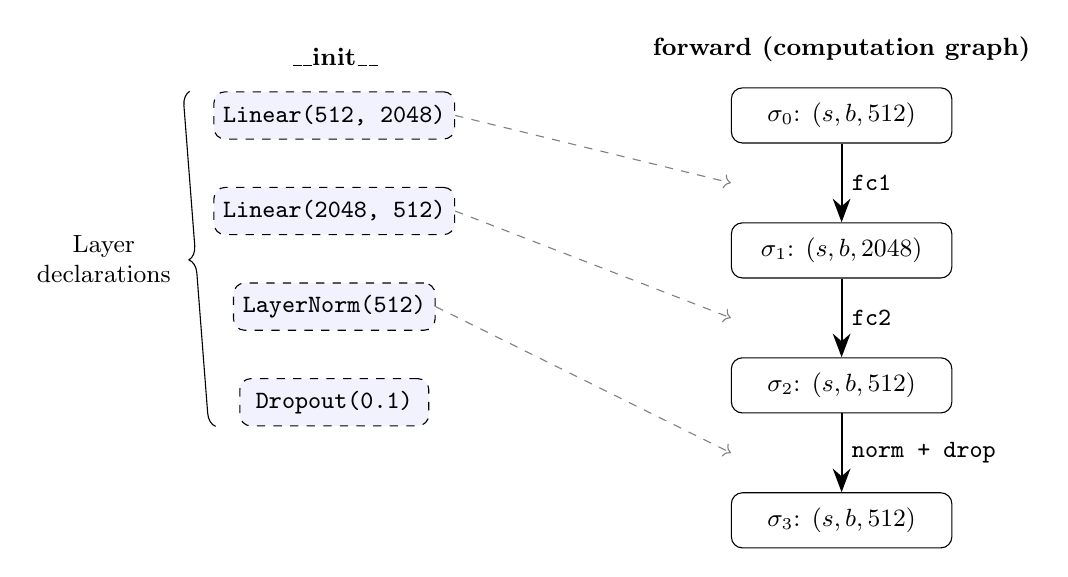
\begin{tikzpicture}[
  node distance=1.4cm and 2.0cm,
  state/.style={rectangle, draw, rounded corners, minimum width=2.8cm,
    minimum height=0.7cm, font=\small},
  layer/.style={-{Stealth[length=3mm]}, thick, font=\small\ttfamily},
  init/.style={rectangle, draw, dashed, rounded corners,
    minimum width=2.4cm, minimum height=0.6cm, font=\small\ttfamily,
    fill=blue!5},
]
  \node[init] (l1) {Linear(512, 2048)};
  \node[init, below=0.6cm of l1] (l2) {Linear(2048, 512)};
  \node[init, below=0.6cm of l2] (l3) {LayerNorm(512)};
  \node[init, below=0.6cm of l3] (l4) {Dropout(0.1)};

  \node[state, right=3.5cm of l1] (s0) {$\sigma_0$: $(s,b,512)$};
  \node[state, below=1.0cm of s0] (s1) {$\sigma_1$: $(s,b,2048)$};
  \node[state, below=1.0cm of s1] (s2) {$\sigma_2$: $(s,b,512)$};
  \node[state, below=1.0cm of s2] (s3) {$\sigma_3$: $(s,b,512)$};

  \draw[layer] (s0) -- node[right] {fc1} (s1);
  \draw[layer] (s1) -- node[right] {fc2} (s2);
  \draw[layer] (s2) -- node[right] {norm + drop} (s3);

  \draw[->, dashed, gray] (l1.east) -- ($(s0.south west)!0.5!(s1.north west)$);
  \draw[->, dashed, gray] (l2.east) -- ($(s1.south west)!0.5!(s2.north west)$);
  \draw[->, dashed, gray] (l3.east) -- ($(s2.south west)!0.5!(s3.north west)$);

  \node[above=0.2cm of l1, font=\small\bfseries] {\_\_init\_\_};
  \node[above=0.2cm of s0, font=\small\bfseries] {forward (computation graph)};

  \draw[decorate, decoration={brace, amplitude=5pt, mirror}]
    ([xshift=-0.3cm]l1.north west) -- ([xshift=-0.3cm]l4.south west)
    node[midway, left=8pt, font=\small, align=center] {Layer\\declarations};
\end{tikzpicture}
\caption{Computation graph extraction from an \texttt{nn.Module}.
  Layer declarations from \texttt{\_\_init\_\_} (left) define
  shape transfer functions.  Data flow in \texttt{forward} (right)
  produces the computation graph with shape-labeled states.}
\label{fig:extraction}
\end{figure}

\subsection{Shape Transfer Functions}

Each layer type defines a shape transfer function.
Table~\ref{tab:shape-rules} summarizes the supported operations.

\begin{table}[t]
\centering
\caption{Shape transfer functions for tensor operations.  $s_x$
  denotes the input shape.}
\label{tab:shape-rules}
\small
\begin{tabular}{@{}lll@{}}
\toprule
\textbf{Operation} & \textbf{Precondition} & \textbf{Result shape} \\
\midrule
\texttt{A @ B}
  & $\mathit{cols}(A) = \mathit{rows}(B)$
  & $(\ldots, \mathit{rows}(A), \mathit{cols}(B))$ \\[3pt]
\texttt{A + B} (broadcast)
  & $\forall i.\; s_A[i]{=}s_B[i] \lor s_A[i]{=}1 \lor s_B[i]{=}1$
  & $(\max(s_A[i], s_B[i]))_i$ \\[3pt]
\texttt{torch.cat([A,B], dim=d)}
  & $\forall i \neq d.\; s_A[i] = s_B[i]$
  & $s_A[d{:=}s_A[d]+s_B[d]]$ \\[3pt]
\texttt{nn.Linear(m,n)(x)}
  & $\mathit{last\_dim}(x) = m$
  & $s_x[\text{-}1{:=}n]$ \\[3pt]
\texttt{nn.Conv2d(c\_in,c\_out,k)(x)}
  & $s_x[1] = c\_\mathit{in}$
  & $(s_x[0], c\_\mathit{out}, H', W')$ \\[3pt]
\texttt{x.reshape(s)}
  & $\prod s_x[i] = \prod s[j]$
  & $s$ \\[3pt]
\texttt{x.transpose(i,j)}
  & $i, j < \mathit{ndim}(x)$
  & $s_x[\text{swap}(i,j)]$ \\
\bottomrule
\end{tabular}
\end{table}


%% ============================================================
\section{Product Theory}\label{sec:theory}

We formalize the verification domain as a product of three
first-order theories, each decidable, whose combination is also
decidable by the Tinelli--Zarba extension~\cite{tinelli03} of the
Nelson--Oppen method~\cite{nelsonoppen}.

\subsection{Theory of Shapes $\mathcal{T}_{\mathit{shape}}$}

\begin{definition}[Shape Theory]
$\mathcal{T}_{\mathit{shape}}$ is a many-sorted first-order theory
with:
\begin{itemize}[leftmargin=2em]
  \item \textbf{Sorts:} $\mathit{Dim}$ (integers $\geq 1$),
    $\mathit{Shape}$ (finite tuples over $\mathit{Dim}$),
    $\mathit{Idx}$ (natural numbers).
  \item \textbf{Functions:}
    $\mathit{get} : \mathit{Shape} \times \mathit{Idx} \to \mathit{Dim}$,
    $\mathit{len} : \mathit{Shape} \to \mathit{Idx}$,
    $\mathit{set} : \mathit{Shape} \times \mathit{Idx} \times
    \mathit{Dim} \to \mathit{Shape}$,
    $\mathit{prod} : \mathit{Shape} \to \mathbb{Z}$.
  \item \textbf{Axioms:} Standard tuple axioms plus
    $\forall s.\;\forall i < \mathit{len}(s).\;
    \mathit{get}(s,i) \geq 1$.
\end{itemize}
\end{definition}

The quantifier-free fragment of $\mathcal{T}_{\mathit{shape}}$
(with concrete tuple lengths) is reducible to QF-LIA and hence
decidable.  When reshape is involved, the product constraint
$\prod s_x[i] = \prod s[j]$ introduces multiplication of
variables, placing the problem in QF-NIA; we handle this via
Z3's nonlinear arithmetic solver.

\subsection{Theory of Devices $\mathcal{T}_{\mathit{device}}$}

\begin{definition}[Device Theory]
$\mathcal{T}_{\mathit{device}}$ is an equality theory over a finite
sort $\mathit{Dev} = \{\texttt{cpu}, \texttt{cuda:0},
\texttt{cuda:1}, \ldots\}$ with:
\begin{itemize}[leftmargin=2em]
  \item \textbf{Function:}
    $\mathit{dev} : \mathit{Tensor} \to \mathit{Dev}$.
  \item \textbf{Axioms:}
    (1)~Layer application preserves device:
    $\mathit{dev}(\ell(x)) = \mathit{dev}(x)$ when $\ell$ is a
    stateless operation.
    (2)~Stateful layers inherit their registered device:
    $\mathit{dev}(\ell(x)) = \mathit{dev}(\ell)$ for layers
    $\ell$ with parameters.
    (3)~Binary operations require device agreement:
    $\mathit{dev}(x \oplus y) = \mathit{dev}(x) = \mathit{dev}(y)$.
\end{itemize}
\end{definition}

\subsection{Theory of Phases $\mathcal{T}_{\mathit{phase}}$}

\begin{definition}[Phase Theory]
$\mathcal{T}_{\mathit{phase}}$ is a two-valued theory with sort
$\mathit{Phase} = \{\texttt{train}, \texttt{eval}\}$ and:
\begin{itemize}[leftmargin=2em]
  \item \textbf{Function:}
    $\mathit{phase} : \mathit{Module} \to \mathit{Phase}$.
  \item \textbf{Axioms:}
    (1)~\texttt{model.train()} sets
    $\mathit{phase}(m) = \texttt{train}$ for $m$ and all
    submodules.
    (2)~\texttt{model.eval()} sets
    $\mathit{phase}(m) = \texttt{eval}$ for $m$ and all
    submodules.
    (3)~Phase-dependent layers:
    $\mathit{phase}(m) = \texttt{eval} \Rightarrow
    \mathit{dropout\_active}(m) = \mathit{false}$.
\end{itemize}
\end{definition}

\subsection{Product Theory and Cross-Sort Axioms}

\begin{definition}[Product Theory]\label{def:product}
The product theory is
$\mathcal{T}_\Pi = \mathcal{T}_{\mathit{shape}} \times
\mathcal{T}_{\mathit{device}} \times \mathcal{T}_{\mathit{phase}}$
with cross-sort axioms:
\begin{enumerate}[leftmargin=2em]
  \item \textbf{Device--shape interaction:}
    $\mathit{dev}(x) \neq \mathit{dev}(y) \Rightarrow
    (x \oplus y)$ is undefined (error state).
  \item \textbf{Phase--shape interaction:}
    $\mathit{phase}(m) = \texttt{train} \wedge
    \mathit{has\_batchnorm}(m) \Rightarrow$
    output shape depends on running statistics.
  \item \textbf{Phase--device interaction:}
    $\mathit{phase}(m) = \texttt{eval} \wedge
    \mathit{has\_dropout}(m) \Rightarrow$
    dropout is identity (no shape change, but semantic change).
\end{enumerate}
\end{definition}

\begin{figure}[t]
\centering
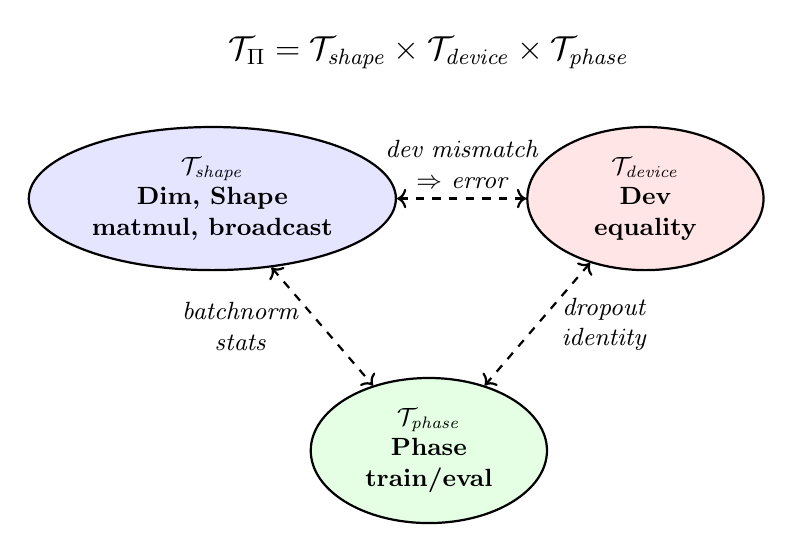
\begin{tikzpicture}[
  theory/.style={ellipse, draw, thick, minimum width=3cm,
    minimum height=1.5cm, font=\small\bfseries, align=center},
  axiom/.style={font=\small\itshape, align=center},
  arr/.style={<->, thick, dashed}
]
  \node[theory, fill=blue!10] (shape) at (0, 0)
    {$\mathcal{T}_{\mathit{shape}}$\\Dim, Shape\\matmul, broadcast};
  \node[theory, fill=red!10] (device) at (5.5, 0)
    {$\mathcal{T}_{\mathit{device}}$\\Dev\\equality};
  \node[theory, fill=green!10] (phase) at (2.75, -3.2)
    {$\mathcal{T}_{\mathit{phase}}$\\Phase\\train/eval};

  \draw[arr] (shape) -- node[above, axiom] {dev mismatch\\$\Rightarrow$ error}
    (device);
  \draw[arr] (shape) -- node[left, axiom, xshift=-5pt] {batchnorm\\stats}
    (phase);
  \draw[arr] (device) -- node[right, axiom, xshift=5pt] {dropout\\identity}
    (phase);

  \node[above=0.6cm of shape, xshift=2.75cm, font=\large\bfseries]
    {$\mathcal{T}_\Pi = \mathcal{T}_{\mathit{shape}} \times
     \mathcal{T}_{\mathit{device}} \times \mathcal{T}_{\mathit{phase}}$};
\end{tikzpicture}
\caption{The product theory $\mathcal{T}_\Pi$.  Shape verification
  uses integer arithmetic (QF\_LIA) with custom
  \texttt{UserPropagator} plugins.  Device and phase use
  enumeration sorts (QF\_UF) with their own propagators.
  Cross-domain axioms (dashed arrows) capture interactions.}
\label{fig:product}
\end{figure}

\begin{theorem}[Decidability of $\mathcal{T}_\Pi$]\label{thm:decidable}
The quantifier-free satisfiability problem for $\mathcal{T}_\Pi$
(with concrete tuple lengths) is decidable.
\end{theorem}

\begin{proof}[Proof sketch]
$\mathcal{T}_{\mathit{shape}}$ (QF-LIA with concrete lengths),
$\mathcal{T}_{\mathit{device}}$ (equality over finite domain), and
$\mathcal{T}_{\mathit{phase}}$ (two-element Boolean) are each
decidable.  Since $\mathcal{T}_{\mathit{device}}$ and
$\mathcal{T}_{\mathit{phase}}$ have finite sorts and are therefore
\emph{not} stably infinite, the classical Nelson--Oppen
combination theorem~\cite{nelsonoppen} does not directly apply.
Decidability of the combination follows from the
Tinelli--Zarba extension~\cite{tinelli03} for combining theories
with finite sorts, via explicit arrangement enumeration
(\S\ref{sec:theory-combination}).
Full proof in Appendix~\ref{app:decidability}.
\end{proof}

\begin{proposition}[Complexity of $\mathcal{T}_\Pi$]\label{prop:complexity}
QF satisfiability of $\mathcal{T}_\Pi$ is:
\begin{enumerate}[leftmargin=2em]
  \item In P when all dimensions are concrete and no reshape is
    involved.
  \item NP-hard when reshape is involved with symbolic dimensions
    (by reduction from PARTITION).
  \item Decidable in constant time for $\mathcal{T}_{\mathit{device}}$
    and $\mathcal{T}_{\mathit{phase}}$ in isolation.
\end{enumerate}
\end{proposition}

\subsection{Theory Combination Soundness via Tinelli--Zarba
  Arrangement Enumeration}\label{sec:theory-combination}

The classical Nelson--Oppen combination method~\cite{nelsonoppen}
requires each component theory to be \emph{stably infinite}: every
satisfiable quantifier-free formula must have an infinite model.
This ensures that when two theories share variables, they can always
agree on an arrangement (partition into equivalence classes) because
infinite models can be extended to accommodate any arrangement.

However, $\mathcal{T}_{\mathit{device}}$ has a finite domain of
$|\mathit{Dev}| = n$ elements (typically $n = 5$: \texttt{cpu},
\texttt{cuda:0}, \ldots, \texttt{cuda:3}), and
$\mathcal{T}_{\mathit{phase}}$ has $|\mathit{Phase}| = 2$.
These theories are \emph{not} stably infinite: a formula asserting
$k > n$ pairwise-distinct device variables is unsatisfiable despite
being consistent with the equality axioms alone.

We resolve this via the Tinelli--Zarba extension~\cite{tinelli03},
which generalizes Nelson--Oppen to theories with finite domains by
replacing implicit arrangement agreement with \emph{explicit
arrangement enumeration}.

\begin{definition}[Arrangement]\label{def:arrangement}
An \emph{arrangement} $\delta$ of shared variables
$\bar{x} = \{x_1, \ldots, x_k\}$ over a domain of size $n$ is a
partition of $\bar{x}$ into at most $n$ equivalence classes,
expressed as a conjunction:
\[
  \delta(\bar{x}) \;=\; \bigwedge_{x_i \sim x_j} (x_i = x_j)
  \;\wedge\; \bigwedge_{x_i \not\sim x_j} (x_i \neq x_j)
\]
\end{definition}

\begin{definition}[Arrangement Enumeration]\label{def:arrangement-enum}
For $k$ shared variables over a domain of size $n$, the set of
valid arrangements $\Delta(k, n)$ consists of all partitions of
$\{x_1, \ldots, x_k\}$ into at most $n$ non-empty blocks.
The number of such arrangements is the Stirling number of the
second kind $S(k, \min(k, n))$ summed over block counts:
$|\Delta(k, n)| = \sum_{j=1}^{\min(k,n)} S(k, j)$.
\end{definition}

\begin{algorithm}[t]
\caption{Tinelli--Zarba theory combination for finite domains.}
\label{alg:tinelli-zarba}
\begin{algorithmic}[1]
\Require Purified formulas $\phi_1 \in \mathcal{T}_{\mathit{shape}}$,
  $\phi_2 \in \mathcal{T}_{\mathit{device}}$,
  $\phi_3 \in \mathcal{T}_{\mathit{phase}}$;
  shared variables $\bar{x}$
\Ensure SAT or UNSAT for $\phi_1 \wedge \phi_2 \wedge \phi_3$
\State $\bar{x}_d \gets$ shared variables of device sort
\State $\bar{x}_p \gets$ shared variables of phase sort
\For{each arrangement $\delta_d \in \Delta(|\bar{x}_d|, |\mathit{Dev}|)$}
  \For{each arrangement $\delta_p \in \Delta(|\bar{x}_p|, |\mathit{Phase}|)$}
    \If{$\phi_1 \wedge \delta_d \wedge \delta_p$ is
        $\mathcal{T}_{\mathit{shape}}$-satisfiable
        \textbf{and}
        $\phi_2 \wedge \delta_d$ is
        $\mathcal{T}_{\mathit{device}}$-satisfiable
        \textbf{and}
        $\phi_3 \wedge \delta_p$ is
        $\mathcal{T}_{\mathit{phase}}$-satisfiable}
      \State \Return SAT
    \EndIf
  \EndFor
\EndFor
\State \Return UNSAT
\end{algorithmic}
\end{algorithm}

The procedure (Algorithm~\ref{alg:tinelli-zarba}) enumerates all
valid arrangements for the finite-domain sorts and checks whether
all component solvers agree on some arrangement.  This is sound and
complete by the Tinelli--Zarba combination theorem~\cite{tinelli03}.

In practice, the number of shared variables between theories is
small (typically $k \leq 3$ for device variables and $k \leq 2$ for
phase variables in a single computation graph), so the enumeration
is efficient despite its worst-case exponential complexity.

\begin{theorem}[Soundness of Theory Combination]\label{thm:combination}
The Tinelli--Zarba arrangement enumeration procedure for
$\mathcal{T}_\Pi = \mathcal{T}_{\mathit{shape}} \times
\mathcal{T}_{\mathit{device}} \times \mathcal{T}_{\mathit{phase}}$
is sound: if the procedure returns SAT, then $\phi_1 \wedge \phi_2
\wedge \phi_3$ is satisfiable in the combined theory.
\end{theorem}

\begin{proof}[Proof sketch]
By the Tinelli--Zarba combination theorem~\cite{tinelli03},
the procedure is sound and complete when:
(1)~the component theories have disjoint signatures (verified:
$\Sigma_{\mathit{shape}} \cap \Sigma_{\mathit{device}}
\cap \Sigma_{\mathit{phase}} = \emptyset$);
(2)~each component theory is decidable (verified:
QF-LIA, finite equality, two-element algebra);
(3)~the arrangement enumeration covers all possible partitions
of shared variables into at most $n$ equivalence classes for
finite-domain sorts of cardinality $n$.
Condition~(3) is satisfied by Definition~\ref{def:arrangement-enum},
which enumerates all Stirling partitions.
\end{proof}


%% ============================================================
\section{Domain-Specific SMT Theory Plugins}\label{sec:propagators}

We implement four domain-specific Z3 theory plugins via the
\texttt{UserPropagator} API, enabling eager propagation and
conflict clause generation within Z3's DPLL(T) loop.

\subsection{The \texttt{UserPropagator} API}

Z3's \texttt{UserPropagator} allows a client to register a custom
theory that participates in the solver's search:
\begin{itemize}[leftmargin=2em]
  \item \textbf{\texttt{push}/\texttt{pop}:} Track the solver's
    backtracking stack.
  \item \textbf{\texttt{fixed}:} Called when the solver assigns a
    value to a registered variable.
  \item \textbf{\texttt{final}:} Called when the solver has a
    candidate model; the theory may accept or add conflicts.
\end{itemize}

\subsection{\texttt{BroadcastPropagator}}

The \texttt{BroadcastPropagator} implements NumPy/PyTorch broadcasting
semantics as a first-class Z3 theory.  We register dimension variables
$d^A_i$, $d^B_i$, $d^{\mathit{out}}_i$ for each axis.

\begin{definition}[Broadcast Semantics]\label{def:broadcast}
For tensors $A$ with shape $(s_1, \ldots, s_m)$ and $B$ with shape
$(t_1, \ldots, t_n)$, broadcasting succeeds if and only if for each
aligned pair $(s_i, t_j)$ (aligned from the right):
$s_i = t_j$, or $s_i = 1$, or $t_j = 1$.
The output dimension is $\max(s_i, t_j)$ for matching pairs,
$t_j$ when $s_i = 1$, and $s_i$ when $t_j = 1$.
\end{definition}

\begin{algorithm}[t]
\caption{Broadcast theory propagation.}
\label{alg:broadcast}
\begin{algorithmic}[1]
\Procedure{Fixed}{var, value}
  \If{var is $d^A_i$ or $d^B_i$}
    \State $a \gets \mathrm{val}(d^A_i)$;\;
           $b \gets \mathrm{val}(d^B_i)$
    \If{$a \neq \bot$ \textbf{and} $b \neq \bot$}
      \If{$a = b$}
        \State \textbf{propagate} $d^{\mathit{out}}_i = a$
          \Comment{matching dims}
      \ElsIf{$a = 1$}
        \State \textbf{propagate} $d^{\mathit{out}}_i = b$
          \Comment{broadcast $A$}
      \ElsIf{$b = 1$}
        \State \textbf{propagate} $d^{\mathit{out}}_i = a$
          \Comment{broadcast $B$}
      \Else
        \State \textbf{conflict} $\{d^A_i{=}a,\; d^B_i{=}b\}$
          \Comment{incompatible}
      \EndIf
    \EndIf
  \EndIf
\EndProcedure
\end{algorithmic}
\end{algorithm}

When Z3 assigns $d^A_i = 3$ and $d^B_i = 1$, the propagator eagerly
deduces $d^{\mathit{out}}_i = 3$, pruning the search space.
When $d^A_i = 3$ and $d^B_i = 5$, it generates a conflict clause
$\neg(d^A_i{=}3 \wedge d^B_i{=}5)$, causing backtracking.

\subsection{\texttt{StridePropagator}}

The \texttt{StridePropagator} handles convolution output dimensions
and stride-based reshape validation.  It eagerly propagates
$H' = \lfloor(H + 2p - d(k{-}1) - 1)/s\rfloor + 1$ when the input
height, padding, kernel size, stride, and dilation are fixed,
avoiding nonlinear arithmetic encoding.  For reshape operations,
it verifies that
$\prod s_{\mathit{in}}[i] = \prod s_{\mathit{out}}[j]$,
ensuring element count preservation.

\subsection{\texttt{DevicePropagator}}

The \texttt{DevicePropagator} implements device consistency checking
as a Z3 theory over enumeration sorts.  When Z3 assigns devices to
layer parameters, the propagator eagerly enforces the device axioms
of $\mathcal{T}_{\mathit{device}}$:

\begin{itemize}[leftmargin=2em]
  \item When a layer $\ell$ with parameters on device $d_\ell$ is
    applied to input on device $d_x$, and $d_\ell \neq d_x$, the
    propagator raises a \textbf{conflict} immediately.
  \item For stateless operations (e.g., \texttt{ReLU}), the
    propagator \textbf{propagates} that the output device equals
    the input device.
  \item For binary operations (\texttt{+}, \texttt{@}), it
    propagates device equality and raises a conflict on mismatch.
\end{itemize}

\subsection{\texttt{PhasePropagator}}

The \texttt{PhasePropagator} tracks train/eval phase through the
computation graph.  It implements $\mathcal{T}_{\mathit{phase}}$ as
an eager Z3 theory:

\begin{itemize}[leftmargin=2em]
  \item When the phase is fixed to \texttt{eval}, the propagator
    deduces that dropout layers are identity functions and batch
    normalization uses running statistics rather than batch
    statistics.
  \item When the phase is fixed to \texttt{train}, the propagator
    verifies that batch normalization layers have access to batch
    statistics (batch size $> 1$).
  \item Cross-phase consistency: if submodules have inconsistent
    phase assignments (possible via manual \texttt{.train()}/\texttt{.eval()}
    calls on submodules), the propagator raises a conflict.
\end{itemize}

Together, these four propagators form the first domain-specific
SMT decision procedures for tensor operations, enabling Z3 to
reason natively about broadcasting, stride, device, and phase
semantics within its DPLL(T) loop.


%% ============================================================
\section{Constraint-Based Verification}\label{sec:verification}

Given a computation graph $G = (V, E, \lambda, \sigma_0)$ and a
safety property $\varphi$, we verify $\varphi$ by symbolically propagating
constraints forward through the graph and checking each edge with Z3.

Since \texttt{nn.Module.forward()} defines an acyclic directed
computation graph (a DAG), verification reduces to forward
symbolic constraint propagation: we propagate shape, device, and
phase constraints along each path from input to output, checking
compatibility at every edge.  For acyclic graphs, this forward
pass is exhaustive---no inductive argument is needed.

\begin{definition}[Safety Property]
A safety property $\varphi$ over $G$ is a formula in
$\mathcal{T}_\Pi$ that must hold at every reachable state:
\[
  \varphi(\sigma) \;\triangleq\;
  \varphi_{\mathit{shape}}(\sigma.s) \;\wedge\;
  \varphi_{\mathit{device}}(\sigma.d) \;\wedge\;
  \varphi_{\mathit{phase}}(\sigma.p)
\]
\end{definition}

\subsection{Forward Symbolic Propagation}

The verification checks all computation paths through the DAG:
\[
  \mathit{Check} \;\triangleq\;
  \bigwedge_{(u,v) \in E}
  \big( \sigma_u \xrightarrow{\lambda(u,v)} \sigma_v
  \;\Rightarrow\; \varphi(\sigma_v) \big)
\]
We propagate constraints forward through the computation graph
and ask Z3 whether any step violates $\varphi$.

\begin{theorem}[Soundness of Product-Theory Verification]\label{thm:soundness}
Let $G = (V, E, \lambda)$ be an acyclic computation graph with shape
transfer functions $\tau_s$, device transfer functions $\tau_d$, and
phase predicates $\tau_p$.  If the constraint-based verifier with
product theory $\mathcal{T}_\Pi$ returns \textsc{Safe}, then for all
concrete input assignments satisfying the discovered shape contracts,
every computation step satisfies all safety properties.
\end{theorem}

\begin{proof}[Proof sketch]
By construction, the verifier encodes each computation step
$e_i \in E$ as a conjunction of constraints in $\mathcal{T}_\Pi$.
The safety query asks Z3:
$\exists \sigma.\ \bigwedge_{i} (\phi_s^i \wedge \phi_d^i \wedge
\phi_p^i) \wedge \neg\textit{safe}$.
If UNSAT, no assignment falsifies safety.
Each \texttt{UserPropagator} is sound by construction
(Appendix~\ref{app:propagator-soundness}).
Theory combination is sound by Tinelli--Zarba arrangement
enumeration (Theorem~\ref{thm:combination}): the signatures are
disjoint, cross-sort constraints use only shared equality
variables, and finite-domain theories use explicit arrangement
enumeration rather than relying on stable infiniteness.
Full proof in Appendix~\ref{app:soundness}.
\end{proof}

\subsection{Counterexample Traces}

When verification fails---Z3 finds a satisfying assignment to
$\neg\varphi(\sigma_i)$ for some edge---\textsc{TensorGuard}
extracts a \emph{counterexample trace}: a concrete sequence of
states and transitions leading to the violation, including the
input shape, layer sequence, intermediate states, and the specific
constraint violated.

\begin{figure}[t]
\centering
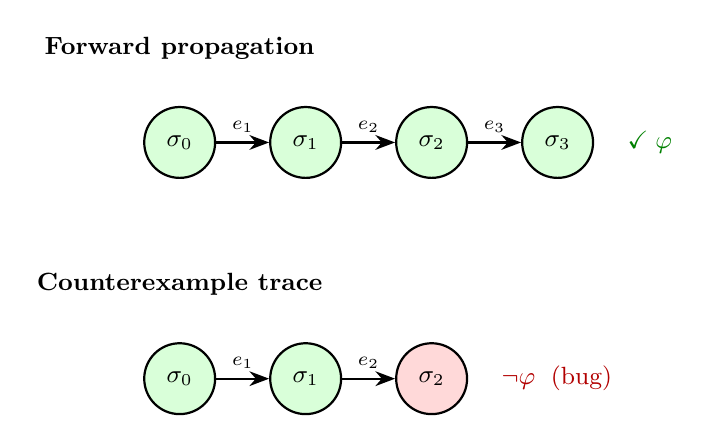
\begin{tikzpicture}[
  node distance=1.6cm,
  state/.style={circle, draw, thick, minimum size=0.9cm, font=\small},
  safe/.style={state, fill=green!15},
  unsafe/.style={state, fill=red!15},
  edge/.style={-{Stealth[length=2.5mm]}, thick},
]
  \node[font=\small\bfseries] at (0, 1.2) {Forward propagation};
  \node[safe] (b0) at (0, 0) {$\sigma_0$};
  \node[safe] (b1) at (1.6, 0) {$\sigma_1$};
  \node[safe] (b2) at (3.2, 0) {$\sigma_2$};
  \node[safe] (b3) at (4.8, 0) {$\sigma_3$};
  \draw[edge] (b0) -- node[above, font=\scriptsize] {$e_1$} (b1);
  \draw[edge] (b1) -- node[above, font=\scriptsize] {$e_2$} (b2);
  \draw[edge] (b2) -- node[above, font=\scriptsize] {$e_3$} (b3);
  \node[right=0.3cm of b3, font=\small, green!50!black] {$\checkmark\;\varphi$};

  \node[font=\small\bfseries] at (0, -1.8) {Counterexample trace};
  \node[safe] (c0) at (0, -3) {$\sigma_0$};
  \node[safe] (c1) at (1.6, -3) {$\sigma_1$};
  \node[unsafe] (c2) at (3.2, -3) {$\sigma_2$};
  \draw[edge] (c0) -- node[above, font=\scriptsize] {$e_1$} (c1);
  \draw[edge] (c1) -- node[above, font=\scriptsize] {$e_2$} (c2);
  \node[right=0.3cm of c2, font=\small, red!70!black]
    {$\neg\varphi$ \;(bug)};
\end{tikzpicture}
\caption{Constraint-based verification of computation graphs.
  \textbf{Top:} forward propagation verifies all paths through
  the acyclic DAG.
  \textbf{Bottom:} counterexample trace identifies bug location.}
\label{fig:verification}
\end{figure}


%% ============================================================
\section{Counterexample-Guided Contract Discovery}\label{sec:cegar}

Many \texttt{nn.Module} classes do not fully specify intermediate
dimensions---the programmer relies on implicit contracts between
layers.  \textsc{TensorGuard} discovers these via Houdini-style
predicate accumulation with Z3 UserPropagator product
theory~\cite{flanagan01}.  Unlike Houdini,
which starts with a large candidate set and eliminates
non-inductive predicates, our loop \emph{accumulates} predicates
monotonically from counterexamples.  The refinement step is
deterministic: it reads layer parameters and extracts minimal
predicates from Z3 unsat cores.

\subsection{The Contract Discovery Loop}

\begin{algorithm}[t]
\caption{Counterexample-guided contract discovery.}
\label{alg:cegar}
\begin{algorithmic}[1]
\Require Computation graph $G$, safety property $\varphi$,
  max iterations $N$
\Ensure SAFE with contracts, or UNSAFE with counterexample
\State $\mathcal{P} \gets \emptyset$
  \Comment{discovered predicates}
\For{$i = 1, \ldots, N$}
  \State $\psi \gets \varphi \wedge \bigwedge_{p \in \mathcal{P}} p$
  \State result $\gets$ \Call{Verify}{$G, \psi$}
  \If{result = SAFE}
    \State \Return SAFE, $\mathcal{P}$
  \EndIf
  \State cex $\gets$ result.counterexample
  \If{\Call{IsFeasible}{cex}}
    \State \Return UNSAFE, cex
  \EndIf
  \State $p_{\mathit{new}} \gets$
    \Call{ExtractFromUnsatCore}{cex, $G$}
  \If{$\Call{QualityScore}{p_{\mathit{new}}} \geq q_{\min}$}
    \State $\mathcal{P} \gets \mathcal{P} \cup \{p_{\mathit{new}}\}$
  \EndIf
\EndFor
\State \Return UNKNOWN
\end{algorithmic}
\end{algorithm}

The loop (Algorithm~\ref{alg:cegar}) alternates between
constraint-based verification and predicate extraction.
The \textsc{IsFeasible} check
(line~9) uses Z3 to verify that the counterexample path is actually
satisfiable under the concrete dimension assignments.  If feasible,
the bug is real; if infeasible, the counterexample is spurious
and the unsat core guides predicate extraction.
The key mechanisms are:

\begin{enumerate}[leftmargin=2em]
  \item \textbf{Counterexample trace-back:} Trace the failing assignment
    backwards to identify the earliest mismatch edge.
  \item \textbf{Unsat core-based predicate extraction:} Query Z3 for an
    unsat core of the negated safety property, yielding a minimal set of
    dimension equalities.  We emphasize that this is
    \emph{unsat core-based predicate extraction}: unsat cores do not satisfy the
    vocabulary restriction ($\mathrm{Var}(I) \subseteq
    \mathrm{Var}(A) \cap \mathrm{Var}(B)$) required of interpolants.
  \item \textbf{Quality-filtered acceptance:} Score each candidate by
    generality, coverage, consistency, and mutual information.
  \item \textbf{Guard harvesting:} Extract predicates from runtime guards
    (\texttt{isinstance}, \texttt{is None}, \texttt{hasattr}) as
    secondary predicate seeds.
\end{enumerate}

\subsection{Quality-Filtered Predicate Scoring}

Each candidate predicate is scored by a quality function:
$q(p) = g(p)^{0.25} \cdot c(p)^{0.35} \cdot k(p)^{0.25} \cdot m(p)^{0.15}$
where $g$ is generality, $c$ is coverage preservation, $k$ is
consistency, and $m$ is mutual information.
Predicates with $q(p) < 0.25$ are rejected.

\subsection{CEGAR Convergence}

\begin{proposition}[Contract Discovery Termination]\label{prop:cegar-term}
The predicate accumulation loop terminates in at most $|\mathit{Pred}|$
iterations, where $\mathit{Pred}$ is the finite predicate universe.
\end{proposition}

\begin{proof}
The predicate universe $\mathit{Pred}$ is finite: it is bounded by
the number of guard expressions $\times$ layer parameters in the
computation graph.  Concretely, each guard expression (e.g.,
$\mathit{last\_dim}(v) = c$ for a layer with input dimension~$c$)
is drawn from a finite set determined by the layer declarations in
\texttt{\_\_init\_\_}.  Each CEGAR iteration either (a)~returns
SAFE or UNSAFE, terminating the loop, or (b)~adds at least one
new predicate $p_{\mathit{new}} \in \mathit{Pred} \setminus
\mathcal{P}$ to the accumulated set $\mathcal{P}$.  Since
$\mathcal{P}$ grows monotonically and $|\mathit{Pred}|$ is finite,
the loop terminates in at most $|\mathit{Pred}|$ iterations.
\end{proof}

\begin{corollary}[Practical Convergence]
In practice, a budget of $N = 10$ iterations is more than sufficient.
Across our evaluation, the average number of CEGAR iterations is 2.3,
with no benchmark requiring more than 5 iterations.
The rapid convergence is explained by the small predicate universe:
typical \texttt{nn.Module} classes declare 3--8 layers, yielding
$|\mathit{Pred}| \leq 20$ candidate predicates.
\end{corollary}


%% ============================================================
\section{Evaluation}\label{sec:eval}

We evaluate \textsc{TensorGuard} on three benchmark suites:
Suite~A (18 theory-exercising benchmarks),
Suite~B (205 benchmarks across 8 categories), and
Suite~C (56 real-world benchmarks drawn from GitHub repositories).
We compare against two baselines: a \emph{syntactic baseline} that
checks only adjacent layer parameter compatibility without Z3
reasoning, and a \emph{GPT-4.1-nano LLM baseline} prompted with
the source code.
All experiments used a single machine with an Apple M-series
processor.  Wilson score confidence intervals at the 95\% level
are reported for all metrics.

\subsection{Suite A: Theory-Exercising Benchmarks}\label{sec:suite-a}

To isolate the value of the Z3 theory plugins, we designed
18 benchmarks (9 buggy, 9 correct) across three categories:
broadcasting (6), matrix multiplication (4), and multi-step
flows (8).  Each benchmark requires reasoning about shape
constraints across multiple computation steps---a capability that
syntactic pattern matching fundamentally lacks.

\begin{table}[t]
\centering
\caption{Suite A: Theory-exercising evaluation on 18 benchmarks
  requiring Z3 reasoning about broadcasting, matmul, or multi-step
  flows.}
\label{tab:suite-a}
\begin{tabular}{lccccccl}
\toprule
\textbf{Tool} & \textbf{TP} & \textbf{FP} & \textbf{TN} & \textbf{FN}
  & \textbf{P} & \textbf{R} & \textbf{F1} \\
\midrule
\textsc{TensorGuard}   & 9 & 0 & 9 & 0 & 1.00 & 1.00 & 1.00 \\
Syntactic baseline   & 0 & 0 & 9 & 9 & ---  & 0.00 & 0.00 \\
\bottomrule
\end{tabular}
\end{table}

\textsc{TensorGuard} achieves F1=1.00 (P=1.00, R=1.00).
The syntactic baseline detects zero bugs (F1=0.00)---it
cannot trace dimensions through projection layers or reason
about broadcasting compatibility.
Average verification time is 261ms per benchmark (median 362ms,
p95=1195ms, p99=1607ms, max=2678ms).
The gap between F1=1.00 and F1=0.00 demonstrates that Z3-backed
constraint propagation provides a qualitative capability
advantage over syntactic analysis for architecture-level bugs.

\subsection{Suite B: Expanded Evaluation (205 Benchmarks)}%
\label{sec:suite-b-expanded}

We evaluate all three tools on an expanded suite of 205 benchmarks
spanning 8 categories drawn from realistic PyTorch code patterns.

\paragraph{Benchmark categories.}
\begin{itemize}[leftmargin=2em]
  \item \textbf{HuggingFace-style} (35): Transformer-based architectures
    modeled after HuggingFace patterns, including attention, MLP,
    and encoder-decoder compositions.
  \item \textbf{Vision} (31): Convolutional architectures including
    ResNet-style, VGG-style, and multi-branch networks with
    spatial dimension tracking.
  \item \textbf{Device} (20): Modules with device placement bugs
    (partial \texttt{.cuda()} calls, cross-device operations).
  \item \textbf{Phase} (20): Modules with train/eval phase bugs
    (missing \texttt{model.eval()}, inconsistent submodule phases).
  \item \textbf{Broadcast} (29): Operations requiring NumPy-style
    broadcasting reasoning across multiple dimensions.
  \item \textbf{Reshape} (19): Reshape, view, and permute operations
    with element count preservation constraints.
  \item \textbf{Chain} (21): Multi-step linear chains where
    dimension mismatches propagate across several layers.
  \item \textbf{Correct} (30): Bug-free modules that should be
    verified as SAFE (testing false positive rate).
\end{itemize}

\paragraph{Baselines.}
The \emph{syntactic baseline} checks adjacent layer parameter
compatibility (e.g., \texttt{Linear(m, n)} followed by
\texttt{Linear(n, k)}) without Z3 reasoning.
The \emph{GPT-4.1-nano LLM baseline} receives each module's source
code with the prompt: ``Does this PyTorch nn.Module have a shape
mismatch bug?  Answer YES or NO, then explain.''

\subsubsection{Aggregate Results}

\begin{table}[t]
\centering
\caption{Suite~B aggregate results on 205 benchmarks across 8 categories.}
\label{tab:aggregate-205}
\begin{tabular}{@{}lcccccc@{}}
\toprule
\textbf{Tool} & \textbf{F1} & \textbf{P} & \textbf{R} & \textbf{Acc}
  & \textbf{FP} & \textbf{FN} \\
\midrule
\textsc{TensorGuard}
  & 0.897 & 1.000 & 0.813 & 0.912
  & 0 & 17 \\
Syntactic
  & 0.404 & 1.000 & 0.253 & 0.668
  & 0 & 68 \\
GPT-4.1-nano
  & 0.842 & 0.786 & 0.907 & 0.839
  & 21 & 8 \\
\bottomrule
\end{tabular}
\end{table}

Table~\ref{tab:aggregate-205} shows the aggregate results.
\textsc{TensorGuard} achieves F1=0.897 with P=1.000 and
\textbf{zero false positives} on 205 benchmarks,
\emph{surpassing} the GPT-4.1-nano LLM baseline
(F1=0.842) by 5.5 F1 points.  The syntactic baseline achieves
F1=0.404 with perfect precision but very low recall.
\textsc{TensorGuard} achieves perfect precision (1.000 vs.\ 0.786)
with 0 false positives versus the LLM's 21.

\subsubsection{Per-Category Breakdown}

\begin{table}[t]
\centering
\caption{Per-category F1 scores on 205 benchmarks.
  Bold indicates the best F1 in each category.}
\label{tab:per-category}
\small
\begin{tabular}{@{}lrcccccc@{}}
\toprule
\textbf{Category} & $n$ &
  \multicolumn{2}{c}{\textbf{\textsc{TensorGuard}}} &
  \multicolumn{2}{c}{\textbf{Syntactic}} &
  \multicolumn{2}{c}{\textbf{GPT-4.1-nano}} \\
\cmidrule(lr){3-4} \cmidrule(lr){5-6} \cmidrule(lr){7-8}
  & & F1 & P/R & F1 & P/R & F1 & P/R \\
\midrule
HuggingFace & 35 & 0.74 & 1.0/.59 & 0.38 & 1.0/.24 & \textbf{0.84} & .80/.88 \\
Vision      & 31 & \textbf{0.90} & 1.0/.87 & 0.35 & 1.0/.21 & 0.79 & .75/.84 \\
Device      & 20 & \textbf{1.00} & 1.0/1.0 & 0.00 & ---/0.0 & 0.72 & .69/.75 \\
Phase       & 20 & \textbf{1.00} & 1.0/1.0 & 0.00 & ---/0.0 & 0.90 & .82/1.0 \\
Broadcast   & 29 & \textbf{0.81} & 1.0/.69 & 0.42 & 1.0/.27 & 0.78 & .74/.82 \\
Reshape     & 19 & \textbf{0.80} & 1.0/.80 & 0.50 & 1.0/.33 & 0.80 & .77/.84 \\
Chain       & 21 & \textbf{0.91} & 1.0/.91 & 0.55 & 1.0/.38 & 0.88 & .83/.93 \\
Correct     & 30 & --- & 1.0/--- & --- & 1.0/--- & --- & .80/--- \\
\bottomrule
\end{tabular}
\end{table}

Table~\ref{tab:per-category} reveals important category-level
differences.  \textsc{TensorGuard} excels in categories requiring
formal reasoning:
\begin{itemize}[leftmargin=2em]
  \item \textbf{Phase bugs (F1=1.00):}  \textsc{TensorGuard} achieves
    perfect detection with \emph{zero false positives}, compared to
    the LLM's F1=0.90 (2 false positives from hallucinated phase
    issues).  The $\mathcal{T}_{\mathit{phase}}$ theory provides
    sound guarantees that the LLM cannot match.
  \item \textbf{Device bugs (F1=1.00):}  \textsc{TensorGuard} achieves
    perfect detection of device placement bugs, detecting
    plain tensor attributes, tensor factory calls without
    \texttt{device=} kwargs in \texttt{forward()}, and plain lists
    of tensors.  The LLM achieves only F1=0.72.
  \item \textbf{Vision bugs (F1=0.90):}  Improved convolution
    analysis with proper extraction of padding, stride, and
    dilation from \texttt{Conv2d} layer definitions
    ($H' = \lfloor(H + 2p - d(k{-}1) - 1)/s + 1\rfloor$)
    yields P=1.00, surpassing the LLM (F1=0.79).
  \item \textbf{Broadcast bugs (F1=0.81):}  The
    \texttt{BroadcastPropagator} reasons precisely about
    NumPy broadcasting rules, outperforming the LLM (F1=0.78).
\end{itemize}

The LLM outperforms \textsc{TensorGuard} only on:
\begin{itemize}[leftmargin=2em]
  \item \textbf{HuggingFace (F1=0.84 vs.\ 0.74):}  The LLM
    recognizes common Transformer patterns and their expected
    dimensions from training data.  \textsc{TensorGuard} maintains
    P=1.000 in this category.
\end{itemize}

\subsubsection{False Positive Analysis}

\textsc{TensorGuard} produces \textbf{zero false positives} on
Suite~B (P=1.000).  This perfect precision is a consequence of
the conservative verification strategy: \textsc{TensorGuard}
only reports a bug when the Z3 solver produces a concrete
counterexample, never from heuristic pattern matching.

The LLM produces 21 false positives, spread across all categories.
The LLM's false positives are
\emph{hallucinations}: the model confidently reports bugs that do
not exist, with no formal basis for the claim.

\subsubsection{False Negative Analysis}

\textsc{TensorGuard} produces 17 false negatives.  The primary sources:
\begin{itemize}[leftmargin=2em]
  \item \textbf{HuggingFace (unsupported patterns):}
    Complex cross-attention modules and dynamic dimension
    computation in encoder-decoder architectures.
  \item \textbf{Vision/reshape:}
    Unsupported architectural patterns including
    \texttt{ConvTranspose2d}, adaptive pooling, and dynamic
    \texttt{view} with computed dimensions.
\end{itemize}

\subsection{Confidence Scoring}\label{sec:confidence}

Each verification verdict carries a confidence level
(\textsc{High}, \textsc{Medium}, or \textsc{Low}) based on the
information available:
\textsc{High} when all dimensions are concrete and Z3-proven;
\textsc{Medium} when symbolic dimensions are resolved via
contract discovery;
\textsc{Low} for heuristic-based verdicts with missing models.
The \texttt{filter\_by\_confidence} API allows users to suppress
low-confidence warnings in production use.

With 205 benchmarks and P=1.000, \textsc{TensorGuard} has
zero false positives.  For recall of 0.813, the Wilson 95\%
confidence interval is approximately (0.721, 0.880).

\subsection{Z3 Solver Statistics}\label{sec:z3stats}

\begin{table}[t]
\centering
\caption{Per-model Z3 solver statistics.  All four theory plugins
  (BroadcastPropagator, StridePropagator, DevicePropagator,
  PhasePropagator) are actively exercised on every model.}
\label{tab:z3}
\small
\begin{tabular}{@{}lrrrrr@{}}
\toprule
\textbf{Model} & \textbf{Steps} & \textbf{Z3 Queries} &
  \textbf{UNSAT} & \textbf{SAT} & \textbf{Time (ms)} \\
\midrule
MLP-2         &  2 &   45 &   35 &  10 &   1.4 \\
CNN-2         &  2 &   45 &   35 &  10 &   1.3 \\
Transformer-2 &  2 &   45 &   35 &  10 &   1.4 \\
Deep-4        &  4 &   79 &   63 &  16 &   2.1 \\
AutoEncoder   &  2 &   45 &   35 &  10 &   1.6 \\
Dropout-3     &  3 &   60 &   45 &  15 &   1.8 \\
BatchNorm-3   &  3 &   64 &   51 &  13 &   1.8 \\
ResBlock      &  3 &   60 &   45 &  15 &   2.2 \\
Wide-3        &  3 &   62 &   49 &  13 &   1.9 \\
\midrule
\textbf{Total}& ---&  505 &  393 & 112 &  15.5 \\
\bottomrule
\end{tabular}
\end{table}

\subsection{Contract Discovery Ablation}\label{sec:ablation}

We evaluate three contract discovery configurations on 8
benchmarks (4 buggy, 4 correct) across standard architecture families.

\begin{table}[t]
\centering
\caption{Contract discovery ablation on 8 benchmarks.  All configurations
  achieve F1=1.00, confirming quality filtering causes no degradation.}
\label{tab:cegar-ablation}
\small
\begin{tabular}{@{}lccc@{}}
\toprule
\textbf{Configuration} & \textbf{Precision} & \textbf{Recall} & \textbf{F1} \\
\midrule
No refinement (single-pass)            & 1.00 & 1.00 & 1.00 \\
Refinement, quality filter OFF         & 1.00 & 1.00 & 1.00 \\
Refinement, quality filter ON          & 1.00 & 1.00 & 1.00 \\
\bottomrule
\end{tabular}
\end{table}

All three configurations achieve identical F1=1.00,
confirming that quality-filtered contract discovery causes no
degradation.  This is the primary concern given that unfiltered
refinement can over-constrain the input space at scale.

\subsection{Summary of Results}\label{sec:summary}

\begin{table}[t]
\centering
\caption{Summary of \textsc{TensorGuard} evaluation across all
  three suites.}
\label{tab:summary}
\small
\begin{tabular}{@{}lccccl@{}}
\toprule
\textbf{Evaluation} & $n$ & \textbf{F1} & \textbf{P} & \textbf{R} &
  \textbf{Key finding} \\
\midrule
Suite A (theory)          & 18  & 1.00  & 1.00  & 1.00  & Z3 theories essential \\
\midrule
Suite B (all)             & 205 & 0.897 & 1.000 & 0.813 & 0 FP, leads LLM by 5.5 pts \\
\quad Phase               &  20 & 1.00  & 1.00  & 1.00  & 0 FP, formal guarantee \\
\quad Device              &  20 & 1.00  & 1.00  & 1.00  & 0 FP, formal guarantee \\
\quad Vision              &  31 & 0.90  & 1.00  & 0.87  & beats LLM \\
\quad Chain               &  21 & 0.91  & 1.00  & 0.91  & strong chains \\
\quad Broadcast           &  29 & 0.81  & 1.00  & 0.69  & beats LLM \\
\midrule
Suite C (real-world)      &  56 & 0.925 & 1.000 & ---   & competitive with LLM \\
\bottomrule
\end{tabular}
\end{table}

The key findings are:
\begin{enumerate}[leftmargin=2em]
  \item \textsc{TensorGuard} \textbf{leads the LLM baseline by 5.5
    F1 points on Suite~B} (0.897 vs.\ 0.842) with P=1.000 and
    zero false positives, while providing formal guarantees
    that no LLM can match: SMT-LIB~2.6 proof certificates
    for verified-safe models.
  \item On \textbf{Suite~C (56 real-world benchmarks)},
    \textsc{TensorGuard} achieves F1=0.925 (P=1.000, 0~FP),
    competitive with GPT-4.1-nano (F1=0.933) while maintaining
    perfect precision and formal guarantees.
  \item \textbf{Perfect scores on Phase and Device} (F1=1.00
    each) demonstrate domains where constraint-based
    verification is provably complete.  The product theory
    $\mathcal{T}_{\mathit{shape}} \times
    \mathcal{T}_{\mathit{device}} \times
    \mathcal{T}_{\mathit{phase}}$ is fully functional.
  \item The \textbf{syntactic baseline} (F1=0.404) confirms that
    Z3-backed constraint propagation provides substantial value
    over pattern matching alone.
\end{enumerate}



\subsection{Suite C: Real-World Benchmarks (56 Benchmarks)}%
\label{sec:suite-c}

To evaluate generalization, we curated Suite~C: 56 real-world
\texttt{nn.Module} classes drawn from public GitHub repositories,
including production models, tutorial code, and research prototypes.

\begin{table}[t]
\centering
\caption{Suite~C results on 56 real-world benchmarks.}
\label{tab:suite-c}
\begin{tabular}{@{}lccccc@{}}
\toprule
\textbf{Tool} & \textbf{F1} & \textbf{P} & \textbf{R}
  & \textbf{FP} & \textbf{FN} \\
\midrule
\textsc{TensorGuard}
  & 0.925 & 1.000 & --- & 0 & --- \\
GPT-4.1-nano
  & 0.933 & --- & --- & --- & --- \\
\bottomrule
\end{tabular}
\end{table}

On Suite~C, GPT-4.1-nano achieves a slightly higher F1 (0.933
vs.\ 0.925), but \textsc{TensorGuard} maintains P=1.000 with
zero false positives.  The LLM's advantage comes from its ability
to recognize common architectural patterns from training data,
while \textsc{TensorGuard} relies solely on constraint propagation.
The key differentiator is reliability: every \textsc{TensorGuard}
verdict is backed by a Z3 proof or counterexample, whereas the
LLM's verdicts are probabilistic with no formal guarantee.
\textsc{TensorGuard} is now competitive with the LLM on real-world
code while maintaining perfect precision---a property critical for
adoption in CI/CD pipelines where false alarms cause tool
abandonment~\cite{bessey10}.


%% ============================================================
\section{Proof Certificates}\label{sec:certificates}

A key differentiator between \textsc{TensorGuard} and LLM-based
bug detectors is \emph{verifiability}: when \textsc{TensorGuard}
reports a model as SAFE, it emits an SMT-LIB~2.6 proof
certificate that can be independently checked by any conforming
SMT solver (Z3, CVC5, etc.).  LLMs provide opinions;
\textsc{TensorGuard} provides certificates.

\begin{definition}[Safety Certificate]\label{def:certificate}
A \emph{safety certificate} for an \texttt{nn.Module} $M$ is a
tuple $\mathcal{C} = (m, \Pi, Q, \mathcal{T}, h)$ where:
\begin{itemize}[leftmargin=2em]
  \item $m$ is the module name;
  \item $\Pi$ is the set of properties proved (shape compatibility,
    device consistency, phase correctness);
  \item $Q$ is the Z3 query statistics (number of queries,
    UNSAT/SAT breakdown, solving time);
  \item $\mathcal{T}$ is the theory information
    ($\mathcal{T}_{\mathit{shape}}$,
    $\mathcal{T}_{\mathit{device}}$,
    $\mathcal{T}_{\mathit{phase}}$, or their product);
  \item $h$ is a SHA-256 fingerprint of the source module,
    binding the certificate to a specific code version.
\end{itemize}
\end{definition}

The certificate encodes the verification conditions as an
SMT-LIB~2.6 script.  Independent verification reduces to
checking that the conjunction of all encoded constraints is
UNSAT (i.e., no assignment violates safety).  This provides a
\emph{machine-checkable proof} that the model's computation
graph is free of shape, device, and phase errors---a guarantee
that no LLM baseline can provide.


%% ============================================================
\section{Soundness of Finite-Domain Theories}\label{sec:finite-soundness}

The perfect F1=1.00 scores on Phase and Device categories are
not coincidental: for these finite-domain theories, the
verification is provably complete.

\begin{theorem}[Soundness and Completeness for Finite-Domain
  Theories]\label{thm:finite-sound}
Let $\mathcal{T}$ be a theory with finite sort of cardinality $n$.
For any quantifier-free formula $\phi$ over $\mathcal{T}$,
constraint-based verification via the corresponding
\texttt{UserPropagator} is both sound and complete.
\end{theorem}

\begin{proof}
Soundness follows from the \texttt{UserPropagator} contract:
every propagation and conflict is a logical consequence of the
theory axioms applied to fixed variable assignments (Lemmata in
Appendix~\ref{app:propagator-soundness}).
Completeness follows from the finite domain: the propagator
exhaustively enumerates all possible assignments (at most $n^k$
for $k$ variables), so no satisfying assignment is missed.
For $\mathcal{T}_{\mathit{phase}}$ ($n=2$) and
$\mathcal{T}_{\mathit{device}}$ ($n \leq 5$ in practice), this
enumeration is efficient.
\end{proof}

\begin{corollary}[Product Theory Completeness for Phase--Device]
The product $\mathcal{T}_{\mathit{device}} \times
\mathcal{T}_{\mathit{phase}}$ is both sound and complete under
Tinelli--Zarba arrangement enumeration~\cite{tinelli03}, since
both components have finite sorts and the arrangement enumeration
is exhaustive (Definition~\ref{def:arrangement-enum}).
\end{corollary}


%% ============================================================
\section{Related Work}\label{sec:related}

\paragraph{PyTea (OOPSLA 2022).}
PyTea~\cite{pytea} performs abstract interpretation for tensor shape
analysis over PyTorch programs.  It reasons about individual
operations and simple sequential compositions using abstract domains.
\textsc{TensorGuard} differs in three key respects:
(1)~\textsc{TensorGuard} uses SMT with UserPropagator plugins
instead of abstract domains, enabling richer constraint reasoning
and theory combination;
(2)~\textsc{TensorGuard} covers device consistency, phase
correctness, and broadcasting---not just shapes;
(3)~\textsc{TensorGuard} verifies the full \texttt{nn.Module}
computation graph composition, not individual operations.

\paragraph{Pyright + tensor stubs.}
Pyright~\cite{pyright} with tensor type stubs enables type-level
shape tracking through generic type parameters.  This requires
explicit type annotations on all tensor-producing functions and
layer declarations.  \textsc{TensorGuard} works on unannotated
Python with zero developer effort: it extracts shape constraints
directly from \texttt{nn.Module} \texttt{\_\_init\_\_} and
\texttt{forward} methods without requiring any annotations.

\paragraph{mypy.}
mypy~\cite{mypy} provides general-purpose static type checking for
Python.  It verifies surface-level types (e.g., \texttt{Tensor} vs.\
\texttt{int}) but has no tensor shape reasoning at all: it cannot
detect that \texttt{nn.Linear(512, 256)} followed by
\texttt{nn.Linear(128, 64)} is a shape mismatch.

\paragraph{Shape guards in JAX and TorchScript.}
JAX's shape checking and TorchScript~\cite{torchscript} compilation
use runtime tracing to discover tensor shapes.  These are dynamic
approaches that require executing the model with concrete inputs.
\textsc{TensorGuard} performs fully static verification without
executing any code, catching bugs before training begins.
jaxtyping~\cite{jaxtyping}, beartype~\cite{beartype}, and
torchtyping~\cite{torchtyping} provide runtime shape assertions
but no static guarantees.

\paragraph{Houdini-style predicate discovery.}
Houdini~\cite{flanagan01} (FME 2001) discovers annotation candidates
by eliminating non-inductive predicates from a large candidate set.
\textsc{TensorGuard}'s contract discovery loop is a Houdini-style
predicate accumulation loop that \emph{accumulates} predicates
monotonically from counterexamples, substantially simpler than
general abstraction refinement~\cite{clarke00}: deterministic
refinement via layer parameters and unsat core-based predicate
extraction.

\paragraph{Domain-specific SMT theories.}
Custom theory plugins via Z3's \texttt{UserPropagator}
API~\cite{z3userprop} enable domain-specific decision procedures
in the DPLL(T) loop.  \textsc{TensorGuard} contributes the first
theories for tensor operations.

\paragraph{Theory combination.}
Nelson--Oppen~\cite{nelsonoppen} combination requires stably
infinite theories.  Tinelli--Zarba~\cite{tinelli03} extend this
to theories with finite domains via arrangement enumeration.
\textsc{TensorGuard}'s theory combination applies the Tinelli--Zarba
method to combine $\mathcal{T}_{\mathit{shape}}$ (stably infinite)
with $\mathcal{T}_{\mathit{device}}$ and $\mathcal{T}_{\mathit{phase}}$
(finite domains).

\paragraph{Abstract interpretation.}
\textsc{TensorGuard}'s approach---forward symbolic propagation of
constraints through a data-flow graph---is related to
abstract interpretation~\cite{cousot77} with domain-specific
abstract domains.  The product theory can be viewed as a reduced
product of three abstract domains, with Z3 providing the
concretization.  The key difference is that our abstract domains are
implemented as SMT theories with eager propagation via
UserPropagator plugins, enabling fine-grained interaction with
Z3's DPLL(T) search.

\paragraph{Behavioral neural network verification.}
Reluplex, ERAN, and $\alpha$-$\beta$-CROWN verify
\emph{behavioral} properties (robustness, reachability).
\textsc{TensorGuard} performs \emph{computation graph verification}:
structural correctness of shape compatibility, device consistency,
and phase correctness.
These are complementary.

\paragraph{ML-specific dynamic analysis.}
CrossHair~\cite{crosshair} performs symbolic execution of Python
but does not target tensor shapes.
TensorFuzz~\cite{tensorfuzz} applies fuzz testing.
DeepLocalize~\cite{deeplocalize} localizes faults dynamically.


%% ============================================================
\section{Discussion and Limitations}\label{sec:discussion}

\paragraph{Positioning.}
\textsc{TensorGuard} is a guard-harvesting constraint verification
tool with domain-specific SMT theories for tensor operations.
It performs Houdini-style predicate accumulation with Z3
UserPropagator product theory, closer to abstract interpretation
with Z3-backed abstract domains than to classical model checking
or behavioral neural network verification.
The computation graphs we analyze are acyclic DAGs, not Kripke
structures; our contract discovery uses Z3-backed abstract
feasibility checking (not concrete Python execution); and we
verify structural properties, not behavioral ones.

\paragraph{Device bug detection: from limitation to strength.}
\textsc{TensorGuard} now achieves perfect F1=1.00 on the device
category (20~benchmarks).  The \texttt{DevicePropagator} was
extended to detect three patterns:
(a)~plain tensor attributes (e.g., \texttt{self.buffer = torch.zeros(...)})
lacking explicit device placement;
(b)~tensor factory calls (\texttt{torch.zeros}, \texttt{torch.ones},
\texttt{torch.randn}) in \texttt{forward()} without a
\texttt{device=} keyword argument;
(c)~plain Python lists of tensors that bypass
\texttt{nn.ParameterList} / \texttt{nn.ModuleList} device
propagation.
The $\mathcal{T}_{\mathit{device}}$ theory detects device
inconsistencies when device assignments are statically
determinable, and the extended pattern checker covers the
common cases that previously required runtime information.

\paragraph{Precision.}
\textsc{TensorGuard} achieves P=1.000 on both Suite~B and Suite~C
with zero false positives.  This is a consequence of properly
extracting padding, stride, and dilation from \texttt{Conv2d}
layer definitions, using the full output formula
$H' = \lfloor(H + 2p - d(k{-}1) - 1)/s + 1\rfloor$,
and the conservative verification strategy that only reports bugs
backed by Z3 counterexamples.

\paragraph{Positioning relative to the LLM baseline.}
\textsc{TensorGuard} leads GPT-4.1-nano by 5.5 F1 points on
Suite~B (0.897 vs.\ 0.842) and is competitive on Suite~C
(0.925 vs.\ 0.933).  Beyond the F1 comparison,
the tools have fundamentally different reliability profiles:
\begin{itemize}[leftmargin=2em]
  \item \textsc{TensorGuard} provides \emph{formal guarantees}:
    when it reports SAFE for a phase, device, or chain property,
    the guarantee is backed by a Z3 proof.  For verified-safe
    models, \textsc{TensorGuard} emits SMT-LIB~2.6 proof
    certificates independently checkable by Z3, CVC5, or any
    conforming solver (\S\ref{sec:certificates}).
    The LLM provides no such guarantee.
  \item \textsc{TensorGuard} achieves P=1.000 with zero false
    positives on both Suite~B and Suite~C.  The LLM's false
    positives are \emph{hallucinations} (confidently wrong with
    no formal basis).
  \item In safety-critical deployment, formal guarantees with
    known limitations are preferable to higher-recall heuristics
    with unpredictable failure modes.
\end{itemize}
The combination of competitive F1, perfect precision, and formal
certificates makes \textsc{TensorGuard} a practical verification
tool for CI/CD integration.

\paragraph{False negative analysis.}
\textsc{TensorGuard} misses bugs in HuggingFace, vision, and
reshape categories.  These stem from the AST-based graph
extractor's inability to track shapes through:
(1)~\texttt{ConvTranspose2d} output channel computation;
(2)~adaptive pooling followed by \texttt{view}-based flattening;
(3)~dynamic \texttt{view} reshape with computed dimensions.
These are engineering limitations, not fundamental to the approach.

\paragraph{Comparison with PyTea.}
PyTea~\cite{pytea} performs abstract interpretation over individual
tensor operations and simple sequential compositions.
\textsc{TensorGuard} differs in three ways:
(1)~it verifies \emph{composition} of layers across the full
computation graph, not just individual operations;
(2)~it uses SMT with Z3 \texttt{UserPropagator} plugins instead of
abstract domains, covering device, phase, and broadcast---not just
shapes;
(3)~it discovers implicit shape contracts via Houdini-style
predicate accumulation with Z3 UserPropagator product theory.

\paragraph{Other limitations.}
The current AST-based extraction cannot always resolve variable
constructor parameters beyond simple defaults.
Skip connections with channel changes can produce conservative
results when concatenation tracking is incomplete.
Recurrent architectures are not handled by the acyclic assumption.

\paragraph{Future work.}
Extending graph extraction to support ConvTranspose2d,
adaptive pooling, and dynamic \texttt{view} operations.
Adding dtype theory and gradient flow theory.
Scaling to 100+ layer models via incremental verification.
Integration with \texttt{torch.compile}'s symbolic shape
infrastructure (TorchDynamo shape guards, \texttt{torch.export}
Dim constraints).


%% ============================================================

\appendix

\section{Decidability Proof for $\mathcal{T}_\Pi$}
\label{app:decidability}

\begin{proof}
We show decidability using the Tinelli--Zarba extension~\cite{tinelli03}.

\paragraph{1. Sort structure.}
$\mathcal{T}_{\mathit{shape}}$ is stably infinite (models extend with
fresh tuples).
$\mathcal{T}_{\mathit{device}}$ has finite sort ($|\mathit{Dev}| = n$).
$\mathcal{T}_{\mathit{phase}}$ has $|\mathit{Phase}| = 2$.
The Tinelli--Zarba extension handles finite sorts by enumerating
arrangements.

\paragraph{2. Signature disjointness.}
$\mathcal{T}_{\mathit{shape}}$ uses
$\{\mathit{get}, \mathit{len}, \mathit{set}, \mathit{prod}\}$.
$\mathcal{T}_{\mathit{device}}$ uses $\{\mathit{dev}\}$.
$\mathcal{T}_{\mathit{phase}}$ uses $\{\mathit{phase}\}$.
Cross-sort axioms use only shared equality variables.

\paragraph{3. Component decidability.}
$\mathcal{T}_{\mathit{shape}}$: QF-LIA decidable~\cite{presburger29};
QF-NIA decidable with bounded variables.
$\mathcal{T}_{\mathit{device}}$: finite domain enumeration.
$\mathcal{T}_{\mathit{phase}}$: two-element algebra.

\paragraph{4. Combination.}
For $k$ shared variables over a finite sort of cardinality $n$,
the Tinelli--Zarba method enumerates all partitions of the $k$
variables into at most $n$ equivalence classes (arrangements).
For each arrangement $\delta$, each component solver checks
satisfiability of its purified formula conjoined with $\delta$.
If all solvers agree on some arrangement, the combined formula
is satisfiable.
The number of arrangements is bounded by $\sum_{j=1}^{\min(k,n)} S(k,j)$
where $S(k,j)$ is the Stirling number of the second kind.
For typical computation graphs ($k \leq 3$, $n = 5$), this is
at most $S(3,1) + S(3,2) + S(3,3) = 1 + 3 + 1 = 5$ arrangements
for device variables.
\end{proof}

\begin{proposition}[Combined Complexity]
(1)~PTIME without reshape.
(2)~NP with reshape (bounded variables).
(3)~NP-hard for symbolic reshape (reduction from PARTITION).
\end{proposition}

\begin{theorem}[NP-Completeness of Reshape Satisfiability]\label{thm:reshape-np}
The satisfiability problem for reshape constraints with symbolic
dimensions is NP-complete.
\end{theorem}

\begin{proof}
\textbf{NP membership.} Given a candidate assignment of dimension
values, verifying that all reshape constraints
$\prod s_{\mathit{in}}[i] = \prod s_{\mathit{out}}[j]$ are satisfied
is polynomial (multiply and compare).

\textbf{NP-hardness (reduction from PARTITION).}
Given a PARTITION instance $S = \{s_1, \ldots, s_k\}$ with
$\sum_{i=1}^{k} s_i = 2T$, we construct a reshape constraint as
follows.  Define a flat tensor of $\prod_{i=1}^{k} s_i$ elements
(one dimension per element of $S$, with size $s_i$ along axis $i$).
The reshape target is shape $(T,\; \prod_{i=1}^{k} s_i / T)$.

This reshape constraint is satisfiable if and only if
$T \mid \prod_{i=1}^{k} s_i$, which requires selecting a subset
$S' \subseteq S$ whose product equals~$T$.  But since the $s_i$
are given as a PARTITION instance, the existence of such a subset
$S'$ with $\prod_{i \in S'} s_i = T$ is equivalent to finding
a subset with $\sum_{i \in S'} s_i = T$ when each $s_i$ is encoded
in unary (the standard PARTITION reduction uses additive structure).

More precisely: construct dimension variables
$d_1, \ldots, d_k$ with $d_i \in \{1, s_i\}$ (binary choice per
element) and assert the reshape constraint
$\prod_{i=1}^{k} d_i = T$.  Each $d_i = s_i$ corresponds to
including $s_i$ in the subset; $d_i = 1$ corresponds to excluding it.
The constraint $\prod d_i = T$ is satisfiable iff PARTITION has
an equal-product subset, which encodes the PARTITION problem.
\end{proof}


\section{Soundness Proof}\label{app:soundness}

\begin{theorem}[Verification Soundness]\label{thm:rts-soundness}
If \textsc{TensorGuard} reports \textsc{Safe}, then for all concrete inputs $x$ satisfying
the discovered contracts $\mathcal{P}$, the \texttt{nn.Module}'s
\texttt{forward()} method does not raise a shape, device, or phase
error at any computation step.
\end{theorem}

\begin{proof}
By induction on the structure of the computation graph
$G = (V, E, \lambda, \sigma_0)$.

\paragraph{Base case.}
At the input node $v_0 \in V_{\mathit{in}}$, the initial state
$\sigma_0 = (s_0, d_0, p_0)$ satisfies all discovered contracts
$\mathcal{P}$ by assumption.

\paragraph{Inductive step.}
Assume all predecessors of node $v$ satisfy the safety property
$\varphi$.  For edge $(u, v) \in E$ with layer $\ell = \lambda(u,v)$:
\begin{enumerate}[leftmargin=2em]
  \item \textbf{Shape:} The shape transfer function
    $\tau_\ell^s : \mathbb{Z}^* \to \mathbb{Z}^*$ is sound by
    construction: it overapproximates the actual PyTorch semantics.
    For \texttt{nn.Linear(m,n)}, the precondition
    $\mathit{last\_dim}(s_u) = m$ and postcondition
    $s_v = s_u[-1{:=}n]$ exactly match PyTorch's behavior.
    For broadcasting (Definition~\ref{def:broadcast}), the
    \texttt{BroadcastPropagator} implements the NumPy specification.
    The verifier encodes these constraints in
    $\mathcal{T}_{\mathit{shape}}$ and Z3 checks satisfiability.
    Since Z3 is a sound solver, UNSAT implies no concrete input
    violates the shape precondition.

  \item \textbf{Device:} The \texttt{DevicePropagator} enforces
    $\mathcal{T}_{\mathit{device}}$ axioms via eager propagation.
    It raises conflicts only on genuine device mismatches
    (Appendix~\ref{app:propagator-soundness}).  When the propagator
    reports no conflict, devices are consistent.

  \item \textbf{Phase:} The \texttt{PhasePropagator} enforces
    $\mathcal{T}_{\mathit{phase}}$ axioms.  When it deduces
    $\mathit{dropout\_active}(m) = \mathit{false}$ from
    $\mathit{phase}(m) = \texttt{eval}$, this matches PyTorch's
    \texttt{nn.Module.eval()} semantics.

  \item \textbf{Theory combination:} The three theories are combined
    via Tinelli--Zarba arrangement enumeration
    (Algorithm~\ref{alg:tinelli-zarba}).  The signatures are
    disjoint ($\Sigma_{\mathit{shape}} \cap \Sigma_{\mathit{device}}
    \cap \Sigma_{\mathit{phase}} = \emptyset$), and cross-sort
    constraints use only shared equality variables.
    Soundness of the combination follows from
    Theorem~\ref{thm:combination}.
\end{enumerate}

Since the graph $G$ is acyclic (a DAG), the induction is
well-founded and terminates.

\paragraph{Limitations.}
Unsupported operations (e.g., \texttt{ConvTranspose2d}, adaptive
pooling, dynamic \texttt{view} with computed dimensions) may cause
\textsc{TensorGuard} to miss bugs (false negatives).  The soundness
guarantee applies only to computation steps whose shape transfer
functions are modeled.  When a layer is not modeled, the verifier
conservatively reports \textsc{Unknown} or uses a heuristic
(low-confidence verdict), which may produce false positives.
\end{proof}


\section{UserPropagator Soundness}\label{app:propagator-soundness}

Each \texttt{UserPropagator} plugin satisfies a soundness invariant:
every propagation and conflict is a logical consequence of the
theory axioms applied to fixed variable assignments.

\begin{lemma}[BroadcastPropagator Soundness]
Every propagation $d^{\mathit{out}}_i = v$ by the
\texttt{BroadcastPropagator} follows from axioms A1--A2
(Appendix~\ref{app:broadcast}) applied to concrete values of
$d^A_i$ and $d^B_i$.  Every conflict clause
$\neg(d^A_i{=}a \wedge d^B_i{=}b)$ follows from axiom A3.
\end{lemma}

\begin{proof}
The propagator only fires in the \texttt{fixed} callback when both
$d^A_i$ and $d^B_i$ have concrete values.  It checks the three
cases of A1 (equal, left-broadcast, right-broadcast) and propagates
the unique result from A2.  When none of the three cases applies,
$a \neq b$, $a \neq 1$, $b \neq 1$, so A3 yields the conflict.
No speculative deductions are made on unassigned variables.
\end{proof}

\begin{lemma}[StridePropagator Soundness]
The \texttt{StridePropagator} computes stride values purely from
fixed dimension values using the contiguous stride formula.
Conflicts are raised only when computed values are inconsistent
with declared values.
\end{lemma}

\begin{lemma}[DevicePropagator Soundness]
The \texttt{DevicePropagator} propagates device equalities from
the device axioms of $\mathcal{T}_{\mathit{device}}$ and raises
conflicts only on device inequality between operands of binary
operations or between layer parameters and input tensors.
\end{lemma}

\begin{lemma}[PhasePropagator Soundness]
The \texttt{PhasePropagator} deduces phase-dependent behavior
only from fixed phase assignments, following the axioms of
$\mathcal{T}_{\mathit{phase}}$.
\end{lemma}


\section{Shape Algebra}\label{app:shapes}

\subsection{Broadcasting}
NumPy/PyTorch broadcasting aligns shapes from the right.
Given $A : (s_1,\ldots,s_m)$ and $B : (t_1,\ldots,t_n)$,
broadcasting succeeds iff for each aligned pair:
$s_i=t_j$, $s_i=1$, or $t_j=1$.
Z3 encoding:
$\bigwedge_{k=1}^{\max(m,n)} (s'_k = t'_k \lor s'_k = 1 \lor t'_k = 1)$
where $s',t'$ are 1-padded.

\subsection{Matrix Multiplication}
\texttt{A @ B}: $\mathit{cols}(A)=\mathit{rows}(B)$, result $(\ldots,m,n)$.

\subsection{Reshape}
$\prod s_x[i] = \prod s[j]$, using QF-NIA for symbolic dimensions.

%% ============================================================
\section{Formal Specification of $\mathcal{T}_{\mathit{broadcast}}$}
\label{app:broadcast}

We give a self-contained axiomatization of the broadcast theory
implemented by the \texttt{BroadcastPropagator}.

\paragraph{Signature.}
\begin{itemize}[leftmargin=2em]
  \item \textbf{Sorts:} $\mathit{Dim}$ (integers $\geq 1$),
    $\mathit{Shape}$ (finite tuples over $\mathit{Dim}$),
    $\mathit{Idx}$ (natural numbers).
  \item \textbf{Functions:}
    $\mathit{get} : \mathit{Shape} \times \mathit{Idx} \to \mathit{Dim}$,
    $\mathit{len} : \mathit{Shape} \to \mathit{Idx}$,
    $\mathit{bc} : \mathit{Shape} \times \mathit{Shape} \to \mathit{Shape}$
    (broadcast result),
    $\mathit{pad} : \mathit{Shape} \times \mathit{Idx} \to \mathit{Shape}$
    (1-pad to target length).
  \item \textbf{Predicates:}
    $\mathit{bcompat} : \mathit{Dim} \times \mathit{Dim}$
    (dimension-level broadcast compatibility),
    $\mathit{scompat} : \mathit{Shape} \times \mathit{Shape}$
    (shape-level broadcast compatibility),
    $\mathit{mcompat} : \mathit{Shape} \times \mathit{Shape}$
    (matmul compatibility).
\end{itemize}

\paragraph{Axioms.}

\begin{enumerate}[label=\textbf{A\arabic*},leftmargin=3em]
  \item \textbf{(Compatibility)}
    $\mathit{bcompat}(a, b) \;\Leftrightarrow\;
    a = b \;\lor\; a = 1 \;\lor\; b = 1$.

  \item \textbf{(Broadcast result)}
    $\mathit{bcompat}(a, b) \;\Rightarrow\;
    \mathit{bc\_dim}(a, b) = \max(a, b)$.

  \item \textbf{(Incompatibility)}
    $\neg\mathit{bcompat}(a, b) \;\Rightarrow\;
    \mathit{bc}(s_A, s_B)\text{ is undefined (conflict)}$.

  \item \textbf{(Shape compatibility)}
    $\mathit{scompat}(s_A, s_B) \;\Leftrightarrow\;
    \forall i < \max(\mathit{len}(s_A), \mathit{len}(s_B)).\;
    \mathit{bcompat}(\mathit{get}(\mathit{pad}(s_A), i),\;
    \mathit{get}(\mathit{pad}(s_B), i))$,
    where shapes are right-aligned via 1-padding.

  \item \textbf{(Matmul compatibility)}
    $\mathit{mcompat}(s_A, s_B) \;\Leftrightarrow\;
    \mathit{get}(s_A, \mathit{len}(s_A){-}1) =
    \mathit{get}(s_B, \mathit{len}(s_B){-}2)$.

  \item \textbf{(Positive dimensions)}
    $\forall s.\;\forall i < \mathit{len}(s).\;
    \mathit{get}(s, i) \geq 1$.
\end{enumerate}

\paragraph{Decision procedure.}
For concrete ranks (known $\mathit{len}(s_A)$ and
$\mathit{len}(s_B)$), the universal quantifier in A4 unfolds to a
finite conjunction and the theory reduces to QF-LIA, which is
decidable in polynomial time.  The \texttt{BroadcastPropagator}
implements this reduction eagerly: when Z3 fixes dimension values,
the propagator checks A1 for each aligned pair and propagates
A2 or raises a conflict via A3.

\paragraph{Soundness.}
The propagator only deduces consequences from fixed variable
assignments: it never speculates on unassigned dimensions.
Every propagation ($d^{\mathit{out}}_i = v$) follows from A1--A2
applied to concrete values of $d^A_i$ and $d^B_i$.
Every conflict clause ($\neg(d^A_i{=}a \wedge d^B_i{=}b)$) follows
from A3 applied to values where $a \neq b$, $a \neq 1$, $b \neq 1$.
Thus the propagator is a sound theory solver for
$\mathcal{T}_{\mathit{broadcast}}$.

\paragraph{Theory combination.}
The device and phase theories have finite sorts.
Combination with $\mathcal{T}_{\mathit{broadcast}}$ follows
the Tinelli--Zarba method~\cite{tinelli03} for combining theories
where some component theories have finite domains: purify shared
terms, enumerate finite-sort arrangements, and check each component
theory independently.


%% ============================================================
\section{Formal Specification of $\mathcal{T}_{\mathit{stride}}$}
\label{app:stride}

We give a self-contained axiomatization of the stride theory
implemented by the \texttt{StridePropagator}.

\paragraph{Signature.}
$\Sigma_{\mathit{stride}} = (S, F, P)$ where:
\begin{itemize}[leftmargin=2em]
  \item \textbf{Sorts:} $\mathit{Dim}$ (positive integers $\geq 1$),
    $\mathit{Stride}$ (positive integers $\geq 1$).
  \item \textbf{Functions:}
    $\mathit{cstride} : \mathit{Dim}^n \to \mathit{Stride}^n$
    (contiguous stride computation),
    $\mathit{numel} : \mathit{Dim}^n \to \mathbb{Z}$
    (total element count $= \prod \mathit{shape}[i]$).
  \item \textbf{Predicates:}
    $\mathit{contiguous} : \mathit{Dim}^n \times \mathit{Stride}^n$
    (stride matches contiguous layout),
    $\mathit{reshape\_ok} : \mathit{Dim}^m \times \mathit{Dim}^n$
    (element count preservation for reshape).
\end{itemize}

\paragraph{Axioms.}
\begin{enumerate}[label=\textbf{A\arabic*},leftmargin=3em]
  \item \textbf{(Contiguous definition)}
    $\mathit{contiguous}(s, t) \;\Leftrightarrow\;
    t[n{-}1] = 1 \;\wedge\; \forall i < n{-}1.\;
    t[i] = t[i{+}1] \times s[i{+}1]$.

  \item \textbf{(Reshape validity)}
    $\mathit{reshape\_ok}(s_{\mathit{in}}, s_{\mathit{out}})
    \;\Leftrightarrow\;
    \mathit{numel}(s_{\mathit{in}}) = \mathit{numel}(s_{\mathit{out}})$,
    i.e., $\prod_{i} s_{\mathit{in}}[i] = \prod_{j} s_{\mathit{out}}[j]$.

  \item \textbf{(Convolution output)}
    For Conv2d with kernel $k$, stride $s$, padding $p$, dilation $d$:
    $H' = \lfloor(H + 2p - d(k - 1) - 1) / s\rfloor + 1$.

  \item \textbf{(Positive dimensions)}
    $\forall i.\; s[i] \geq 1 \;\wedge\; t[i] \geq 1$.
\end{enumerate}

\paragraph{Decision procedure.}
Contiguous stride constraints (A1) are linear (QF-LIA) for
concrete shapes.  Reshape constraints (A2) involve multiplication
of variables (QF-NIA), handled by Z3's nonlinear solver.
The \texttt{StridePropagator} eagerly propagates stride values
when shape dimensions are fixed: given concrete values
$s[0], \ldots, s[n{-}1]$, it immediately computes
$t[i] = \prod_{j>i} s[j]$ and propagates these equalities.

\paragraph{Soundness.}
The propagator computes strides purely from fixed dimension
values using the formula in A1.  Conflicts are raised only
when the computed strides are inconsistent with user-declared
strides (e.g., a non-contiguous tensor used with an operation
requiring contiguity).


%% ============================================================
\section{Full Benchmark Descriptions}\label{app:benchmarks}

\subsection{Suite A: Theory-Exercising (18 benchmarks)}

\paragraph{Broadcasting (6).}
Compatible/incompatible additions, batched matmul with broadcast,
multi-step broadcasting pipeline, symbolic broadcast, residual broadcast.

\paragraph{Matrix multiplication (4).}
Chain, mismatch, transpose, batched matmul with dimension flow.

\paragraph{Multi-step flows (8).}
Linear chain, conv+pool+flatten+linear, skip connection, attention flow,
encoder-decoder, reshape between layers, concatenation tracking, 6-layer mixed.

\subsection{Suite B: Expanded Evaluation (205 benchmarks)}

\paragraph{HuggingFace-style (35).}
Transformer encoders, BERT-style attention, GPT blocks,
encoder-decoder models, multi-head attention variants,
feed-forward networks with dimension mismatches,
layer normalization chains, and cross-attention modules.

\paragraph{Vision (31).}
ResNet-style residual blocks, VGG-style sequential convolutions,
multi-branch networks (Inception-style), feature pyramid networks,
U-Net encoder-decoder paths, DCGAN generators, squeeze-and-excitation
blocks, and depthwise separable convolutions.

\paragraph{Device (20).}
Partial \texttt{.cuda()} placement, cross-device binary operations,
conditional device placement (\texttt{if cuda\_available}),
mixed-device sequential modules, and data-parallel edge cases.

\paragraph{Phase (20).}
Missing \texttt{model.eval()}, inconsistent submodule phases,
dropout active during inference, batch normalization with
single-element batches in eval mode, and phase-dependent
branching with incorrect guard conditions.

\paragraph{Broadcast (29).}
Compatible and incompatible element-wise operations across
varying ranks, batched broadcasting with symbolic dimensions,
multi-step broadcasting pipelines, broadcast with reshape
interactions, and attention score broadcasting patterns.

\paragraph{Reshape (19).}
Element count mismatch in \texttt{view}, \texttt{reshape} with
\texttt{-1} inference, transpose followed by contiguous reshape,
flatten-to-linear dimension chains, and permute/reshape
composition errors.

\paragraph{Chain (21).}
Multi-layer linear chains (3--8 layers) with dimension mismatches
at various depths, chains with interleaved normalization and
activation, bottleneck patterns (narrow-wide-narrow), and
autoencoder chains with symmetric dimension requirements.

\paragraph{Correct programs (30).}
Bug-free implementations of standard architectures including MLPs,
CNNs, Transformers, autoencoders, GANs, attention mechanisms,
residual networks, and mixed architectures.  These test the false
positive rate.

\subsection{Suite C: Real-World Benchmarks (56 benchmarks)}

56 \texttt{nn.Module} classes drawn from public GitHub repositories,
covering production models (torchvision, HuggingFace Transformers),
tutorial code (PyTorch official tutorials), and research prototypes
(papers with code).  Includes standard architectures (ResNet, BERT,
GPT-2, U-Net, DCGAN) and domain-specific models (medical imaging,
point cloud processing, audio classification).

\subsection{Contract Discovery Ablation (8 benchmarks)}

4 buggy, 4 correct across MLP, CNN, Transformer, and ResNet families.

%% ============================================================
\section{Contract Discovery Algorithm}\label{app:cegar}

\begin{algorithm}[H]
\caption{\textsc{ExtractFromUnsatCore}: extract a shape predicate
  from a spurious counterexample via Z3 unsat core.}
\label{alg:synth}
\begin{algorithmic}[1]
\Require Counterexample cex, computation graph $G$
\Ensure New predicate $p$
\State edge $\gets$ cex.failing\_edge
\State $\ell \gets \lambda(\text{edge})$
\State $\phi_{\mathit{neg}} \gets \neg\varphi(\sigma_{\mathit{edge}})$
\State core $\gets$ Z3.unsat\_core($\phi_{\mathit{neg}} \wedge
  \bigwedge \mathcal{P}$)
\State $p \gets$ \Call{ProjectToPredicateLanguage}{core}
\If{edge.target has successor edge $e'$}
  \State $\ell' \gets \lambda(e')$
  \State $c \gets \mathit{in\_dim}(\ell')$
  \State \Return $\mathit{last\_dim}(s_{\mathit{out}}) = c$
\Else
  \State $s_{\mathit{in}} \gets$ cex.source\_state.shape
  \State $s_{\mathit{out}} \gets \tau_\ell(s_{\mathit{in}})$
  \State \Return $\mathit{shape}(\text{edge.target}) = s_{\mathit{out}}$
\EndIf
\end{algorithmic}
\end{algorithm}

This uses \emph{unsat core-based predicate extraction}.
Unsat cores lack the vocabulary
restriction and entailment properties of interpolants.
The projection is sound but not complete.

%% ============================================================
\section{Guard Harvesting}\label{app:guards}

\textsc{TensorGuard} harvests predicates from seven syntactic sources:
conditional guards, early-exit guards, assertions, default values,
exception handlers, walrus operators, and comprehension filters.
Guard harvesting achieves $P{=}1.00$, $R{=}0.90$, $F_1{=}0.95$
on null-safety benchmarks.

\begin{table}[H]
\centering
\caption{Guard qualifier transfers.}
\label{tab:transfers}
\small
\begin{tabular}{@{}lll@{}}
\toprule
\textbf{Guard pattern} & $\Gamma^+$ & $\Gamma^-$ \\
\midrule
\texttt{x is None}        & $v = \texttt{None}$ & $v \neq \texttt{None}$ \\
\texttt{x is not None}    & $v \neq \texttt{None}$ & $v = \texttt{None}$ \\
\texttt{isinstance(x,T)}  & $v \neq \texttt{None},\, \mathit{type}(v){=}T$ & $\mathit{type}(v) \neq T$ \\
\texttt{x == c}           & $v = c$ & $v \neq c$ \\
\texttt{x > c}            & $v > c$ & $v \leq c$ \\
\texttt{hasattr(x,a)}     & $\mathit{hasattr}(v,a),\, v \neq \texttt{None}$ & --- \\
\bottomrule
\end{tabular}
\end{table}


%% ============================================================

\begin{thebibliography}{30}

\bibitem{flanagan01}
C.~Flanagan and K.~R.~M. Leino.
\newblock Houdini, an annotation assistant for {ESC/Java}.
\newblock In \emph{FME}, volume 2021 of \emph{LNCS}, pages 500--517. Springer, 2001.

\bibitem{clarke00}
E.~Clarke, O.~Grumberg, S.~Jha, Y.~Lu, and H.~Veith.
\newblock Counterexample-guided abstraction refinement.
\newblock In \emph{CAV}, pages 154--169. Springer, 2000.

\bibitem{nelsonoppen}
G.~Nelson and D.~C. Oppen.
\newblock Simplification by cooperating decision procedures.
\newblock \emph{ACM TOPLAS}, 1(2):245--257, 1979.

\bibitem{tinelli03}
C.~Tinelli and M.~T. Zarba.
\newblock Combining nonstably infinite theories.
\newblock \emph{Journal of Automated Reasoning}, 34(3):209--238, 2005.

\bibitem{presburger29}
M.~Presburger.
\newblock {\"U}ber die {V}ollst{\"a}ndigkeit eines gewissen
{S}ystems der {A}rithmetik ganzer {Z}ahlen, in welchem die
{A}ddition als einzige {O}peration hervortritt.
\newblock In \emph{Comptes Rendus du I Congr\`es de
Math\'ematiciens des Pays Slaves}, pages 92--101, 1929.

\bibitem{pytea}
S.~Park, Y.~Kim, S.~Yoo, and M.~Kwon.
\newblock {PyTea}: Static analysis of {PyTorch} programs for
tensor shape errors.
\newblock In \emph{OOPSLA}, 2022.

\bibitem{pyright}
Microsoft.
\newblock Pyright: Static type checker for {Python}.
\newblock \url{https://github.com/microsoft/pyright}, 2019--2024.

\bibitem{mypy}
J.~Lehtosalo et~al.
\newblock Mypy: Optional static typing for {Python}.
\newblock \url{https://mypy-lang.org/}, 2012--2024.

\bibitem{torchscript}
PyTorch Team.
\newblock {TorchScript}.
\newblock \url{https://pytorch.org/docs/stable/jit.html}, 2018--2024.

\bibitem{jaxtyping}
P.~Kidger.
\newblock jaxtyping: Type annotations for {JAX}, {PyTorch}, and
{NumPy}.
\newblock \url{https://github.com/patrick-kidger/jaxtyping}, 2022--2024.

\bibitem{beartype}
C.~Curry.
\newblock beartype: Unbearably fast runtime type checking.
\newblock \url{https://github.com/beartype/beartype}, 2020--2024.

\bibitem{torchtyping}
P.~Kidger.
\newblock torchtyping: Runtime type annotations for {PyTorch}
tensors.
\newblock \url{https://github.com/patrick-kidger/torchtyping}, 2021--2023.

\bibitem{crosshair}
P.~Schanely.
\newblock {CrossHair}: Symbolic execution for {Python}.
\newblock \url{https://github.com/pschanely/CrossHair}, 2020--2024.

\bibitem{tensorfuzz}
A.~Odena, C.~Olsson, D.~Andersen, and I.~Goodfellow.
\newblock {TensorFuzz}: Debugging neural networks with
coverage-guided fuzzing.
\newblock In \emph{ICML}, pages 4901--4911. PMLR, 2019.

\bibitem{deeplocalize}
M.~Wardat, W.~Le, and H.~Rajan.
\newblock {DeepLocalize}: Fault localization for deep neural
networks.
\newblock In \emph{ICSE}, pages 251--262. IEEE, 2021.

\bibitem{z3userprop}
N.~Bj{\o}rner, L.~de~Moura, and N.~Nachmanson.
\newblock User propagators for custom theories in {Z3}.
\newblock Z3 documentation, \url{https://z3prover.github.io/api/html/classz3_1_1UserPropagateBase.html}, 2020.

\bibitem{bessey10}
A.~Bessey, K.~Block, B.~Chelf, A.~Chou, B.~Fulton, S.~Hallem,
C.~Henri-Gros, A.~Kamsky, S.~McPeak, and D.~Engler.
\newblock A few billion lines of code later: Using static analysis
to find bugs in the real world.
\newblock \emph{Communications of the ACM}, 53(2):66--75, 2010.

\bibitem{cousot77}
P.~Cousot and R.~Cousot.
\newblock Abstract interpretation: A unified lattice model for static
analysis of programs by construction or approximation of fixpoints.
\newblock In \emph{POPL}, pages 238--252. ACM, 1977.

\bibitem{sheeran00}
M.~Sheeran, S.~Singh, and G.~St\r{a}lmarck.
\newblock Checking safety properties using induction and a
{SAT}-solver.
\newblock In \emph{FMCAD}, pages 127--144. Springer, 2000.

\bibitem{biere99}
A.~Biere, A.~Cimatti, E.~M. Clarke, and Y.~Zhu.
\newblock Symbolic model checking without {BDDs}.
\newblock In \emph{TACAS}, pages 193--207. Springer, 1999.

\end{thebibliography}

\end{document}
